\documentclass[compress]{beamer}
\usepackage[utf8]{inputenc}
%!TEX encoding = UTF-8 Unicode
\usepackage{amsmath}
\usepackage{amsfonts}
\usepackage{amssymb}
\usepackage[american]{babel}
\usepackage{xspace}
\usepackage{graphicx,psfrag}
\usepackage{CJK}
\usepackage{rotating}
\usepackage{pstool}
\usepackage{ifthen}
\usepackage{figlatex}


\graphicspath{{fig/}}


\mode<presentation>
{
  \usetheme{Replica}
  \setbeamercovered{transparent}
%  \setbeamertemplate{mini frames}[tick]
%  \setbeamertemplate{mini frame in other subsection}{}
}

\makeatletter
\let\beamer@writeslidentry@miniframeson=\beamer@writeslidentry
\def\beamer@writeslidentry@miniframesoff{%
  \expandafter\beamer@ifempty\expandafter{\beamer@framestartpage}{}% does not happen normally
  {%else
    % removed \addtocontents commands
    \clearpage\beamer@notesactions%
  }
}
\newcount\beamer@writeslidentry@miniframesoneoversome@counter
\newcount\beamer@writeslidentry@miniframesoneoversome@limit
\beamer@writeslidentry@miniframesoneoversome@counter=1
\newcount\beamer@writeslidentry@miniframesoneoversome@limit
\beamer@writeslidentry@miniframesoneoversome@limit=5
\def\beamer@writeslidentry@miniframesoneoversome{%
  \ifnum\beamer@writeslidentry@miniframesoneoversome@counter=\beamer@writeslidentry@miniframesoneoversome@limit\relax%
    \beamer@writeslidentry@miniframesoneoversome@counter=1\relax%
    \beamer@writeslidentry@miniframeson%
  \else%
    \advance\beamer@writeslidentry@miniframesoneoversome@counter by 1%
    \beamer@writeslidentry@miniframesoff%
  \fi%
}
\newcommand*{\miniframeson}{\let\beamer@writeslidentry=\beamer@writeslidentry@miniframeson}
\newcommand*{\miniframesoff}{\let\beamer@writeslidentry=\beamer@writeslidentry@miniframesoff}
\newcommand*{\miniframesalternate}[1]{%
   \beamer@writeslidentry@miniframesoneoversome@counter=1\relax%
   \beamer@writeslidentry@miniframesoneoversome@limit=#1\relax%
   \let\beamer@writeslidentry=\beamer@writeslidentry@miniframesoneoversome}

% Define the subsectionsonly option for beamer toc
\def\beamer@tocaction@only#1{\only<.(1)>{\usebeamertemplate**{#1}}}
\define@key{beamertoc}{subsectionsonly}[]{\beamer@toc@subsectionstyle{show/only}\beamer@toc@subsubsectionstyle{show/shaded/hide}}
\makeatother


\usepackage{relsize}
\usepackage{wasysym}
\def\smiley{\green{\larger[2]\wasyfamily\char44}\xspace}
\def\frownie{\blue{\larger[2]\wasyfamily\char47}\xspace}
\def\quesley{\yyellow{\hbox to -0.08em{\textraiseglotstop}$_{\textrm{\wasyfamily\char47}}$}\xspace}


%% Macros
\newcommand{\probaSymbol}{\mathbb P}
\newcommand{\proba}[1]{\probaSymbol\left(#1\right)}
\newcommand{\esperance}[1]{\mathbb E\left(#1\right)}
\newcommand{\Psachant} [2]{\mathbb P\left(#1\left|\,\vphantom{#1} #2\right.\right)} %proba de #1 sachant #2
\newcommand{\Esachant} [2]{\mathbb E\left(#1\left|\,\vphantom{#1} #2\right.\right)} %proba de #1 sachant #2


\newcommand<>{\blue}[1]{{\color#2{blue!100!black!100}#1}}
\newcommand<>{\redd}[1]{{\color#2{red!80!black}#1}}
\newcommand<>{\green}[1]{{\color#2{green!70!black}#1}}
\newcommand<>{\purple}[1]{{\color#2{blue!50!red}#1}}
\newcommand{\red}[1]{\textcolor{red}{#1}\xspace}
\title[Cooperative Checkpointing]{Optimal Cooperative Checkpointing for Shared High-Performance Computing Platforms}

\usepackage{xcolor,soul}
\sethlcolor{green}
\definecolor{cinnabar}{rgb}{1,0.5,0.5}
\makeatletter
\newcommand\SoulColor{%
  \let\set@color\beamerorig@set@color
  \let\reset@color\beamerorig@reset@color}
\makeatother
\usepackage[most]{tcolorbox}
\newtcolorbox{myblock}[2][]{beamer,title=#2,fonttitle=\sffamily,
  left=1mm,right=1mm,top=1mm,bottom=1mm,arc=2mm,
  colback=black,colupper=white,colframe=yellow,
  coltitle=black,title style={top color=red!70,bottom color=yellow},
  #1}

\usepackage{gnuplot-lua-tikz}
\newcommand{\muind}{\mu_{\text{ind}}}
\newcommand{\bandtotal}{\beta_{\text{tot}}}
\newcommand{\bandavail}{\beta_{\text{avail}}}
\newcommand{\appset}{{\mathcal A}}
\newcommand{\nbnodesplat}{{\mathcal N}}
\newcommand{\nbapps}{|{\mathcal A}|}
\newcommand{\app}[1]{A_{#1}}
\newcommand{\application}[2]{a_{#1}^{#2}}
\newcommand{\nbapp}[1]{n_{#1}}
\newcommand{\nbnodes}[1]{q_{#1}}
\newcommand{\period}[1]{P_{#1}}
\newcommand{\ckpt}[1]{C_{#1}}
\newcommand{\reco}[1]{R_{#1}}
\newcommand{\size}[1]{\mathit{size}_{#1}}
\newcommand{\wasteapp}[1]{W_{#1}}
\newcommand{\wap}[1]{W_{#1}}
\newcommand{\wapp}[2]{W_{#1}(#2)}
\newcommand{\mtbfplat}{\mu}
\newcommand{\wasteplat}{W}
\newcommand{\wasteplatt}{\textsc{Waste}\xspace}
\newcommand{\opt}{{\textit opt}}
\newcommand{\lost}{{\textit lost}}
\newcommand{\EE}{{\mathbb E}}
\newcommand{\ioconstraint}{F}
\newcommand{\lastckpt}[2]{L_{#1}^{#2}}
\newcommand{\wastefct}[2]{W_{#1}(#2)}
\newcommand{\pool}{{\mathcal P}}
\newcommand{\risk}{{\textsc Risk}}
%\newcommand{\todo}[1]{\textit{TBD: [#1]}}
\newcommand{\dca}[1]{\todo[inline]{DCA: #1}}
\newcommand{\kbf}[1]{\todo[inline]{kbf: #1}}

\newcommand{\IOcat}{\textsc{IO-Candidate}\xspace}
\newcommand{\Ckptcat}{\textsc{Ckpt-Candidate}\xspace}
\newcommand{\Catiocat}{\mathcal{C}_{IO}\xspace}
\newcommand{\Catckptcat}{\mathcal{C}_{Ckpt}\xspace}

\newcommand{\nocoop}{\emph{Oblivious}\xspace}
\newcommand{\fifoblock}{\emph{Ordered}\xspace}
\newcommand{\fifononblock}{\emph{Ordered-NB}\xspace}
\newcommand{\leastwaste}{\emph{Least-Waste}\xspace}

\def\propfixed{\nocoop-Fixed\xspace}
\def\propdaly{\nocoop-Daly\xspace}
\def\bfifofixed{\fifoblock-Fixed\xspace}
\def\bfifodaly{\fifoblock-Daly\xspace}
\def\fifofixed{\fifononblock-Fixed\xspace}
\def\fifodaly{\fifononblock-Daly\xspace}
\def\cooperative{\leastwaste}



\subtitle{}

\author[yves.robert@inria.fr]{%
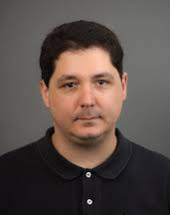
\includegraphics[width=1.17cm]{photos/thomas.jpg}
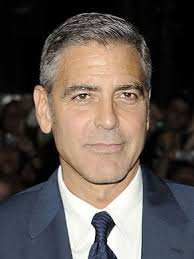
\includegraphics[width=0.8cm]{photos/clooney.jpg}
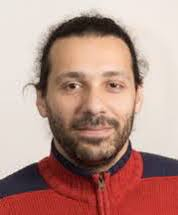
\includegraphics[width=1.14cm]{photos/aurelien.jpg}
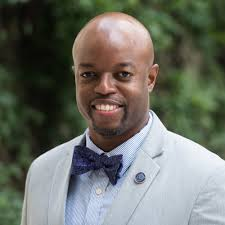
\includegraphics[width=1.07cm]{photos/dorian.jpg}
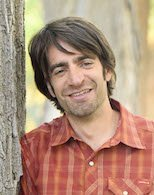
\includegraphics[width=0.9cm]{photos/kurt.jpg}
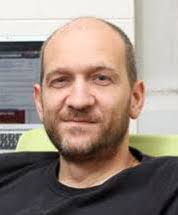
\includegraphics[width=1.16cm]{photos/george.jpg}
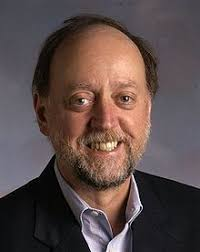
\includegraphics[width=0.85cm]{photos/jack.jpg}\\
~\\
{\footnotesize
Thomas Hérault$^{1}$,
\textcolor{red}{Yves Robert}$^{1,2}$ 
Aurélien Bouteiller$^{1}$,\\
Dorian Arnold$^{3}$,
Kurt Ferreira$^{4}$,
George Bosilca$^{1}$,
Jack Dongarra$^{1}$\\
}
{\tiny
~\\
1. University of Tennessee Knoxville, USA\\
2. Laboratoire LIP, ENS Lyon \& Inria, France\\
3. Emory University, Atlanta, GA, USA\\
4. Sandia National Laboratory, USA\\
}}


\date[March 12, 2018]{\textcolor{green}{Inria Bordeaux -- March 12, 2018}}

\AtBeginSection[]
{
  \begin{frame}<beamer>
    \frametitle{Outline}
     {\scriptsize
       \tableofcontents[sectionstyle=show/shaded,subsectionstyle=show/show/hide]
    }
  \end{frame}
}

\AtBeginSubsection[]
{
  \begin{frame}<beamer>
    \frametitle{Outline}
     {\scriptsize
       \tableofcontents[sectionstyle=show/shaded,subsectionstyle=show/shaded/hide]
    }
  \end{frame}
}

\begin{document}

\miniframesalternate{5}
\pgfaliasimage{figbackground}{figbackground-orange}% !!!

\begin{frame}
  \titlepage
\end{frame}


\begin{frame}
  \frametitle{Framework}

\begin{itemize}
\item \green{Space-sharing} prevalent in HPC platforms
\item Application instances:
\begin{itemize}
\item have dedicated computational nodes
\item share interconnect links and storage partition (PFS)
\item checkpoint (to stable storage) independently
\end{itemize}
$\Rightarrow$ \redd{network and storage contention}
\end{itemize}

\end{frame}

\section{Checkpointing 101}


\begin{frame}
  \frametitle{Checkpointing 101}


When do applications checkpoint on HPC systems?
\begin{itemize}
\item Standard practice:  every hour 
\item State-of-the-art: Young/Daly period
\end{itemize}


\end{frame}

\frame{
    \frametitle{Platform MTBF (1/2)}


\centering
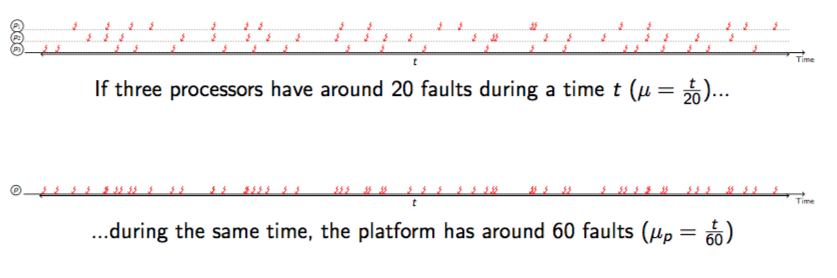
\includegraphics[width=11cm]{photos/faults.png}

}

\frame{
    \frametitle{Platform MTBF (2/2)}


\begin{itemize}
\item Rebooting only faulty processor
\item Platform failure distribution\\
$\Rightarrow$ superposition of $p$ IID processor distributions\\
$\Rightarrow$ IID only for Exponential\\
\item Platform of $p$ processors:
\begin{itemize}
\item $n_{p}(F)$ = number of platform failures until time $F$
\item$\lim_{F \rightarrow +\infty} \frac{F}{n_{p}(F)} \stackrel{\text{def}}{=} \mu_{p}$
\end{itemize}
\end{itemize}


\red{$$\textbf{Theorem: } \mu_{p} = \frac{\muind}{p} \text{ for arbitrary 
distributions}$$}

}

\frame{
    \frametitle{Optimal checkpointing period (1/3)}


\begin{center}
%\vspace{-2.5mm}
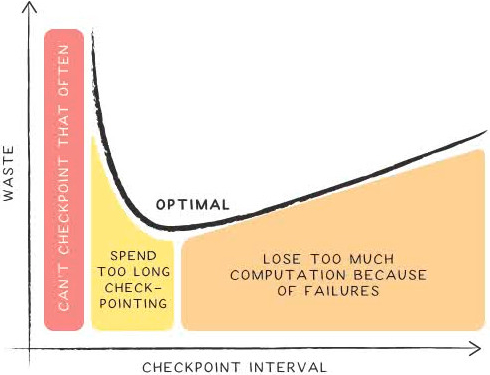
\includegraphics[width=0.65\textwidth]{photos/resilience.jpg}
\end{center}

}


\frame{
    \frametitle{Optimal checkpointing period (2/3)}

\noindent
With period $T$:

\vfill
$$\wasteplatt = \frac{C}{T} \oplus \frac{1}{\mu} (D+R+\frac{T}{2})$$

\vfill
$$\redd{T_{\opt} = \sqrt{2 C \mu}} \qquad \green{\text{(Young/Daly)}}$$
$$\wasteplatt_{\opt} = \frac{2C}{\mu}$$

}


\frame{
    \frametitle{Optimal checkpointing period (3/3)}


$$\begin{array}{ll}
\EE(W) & = e^{-\lambda (W+C)} (W+C)\\
& + (1-  e^{-\lambda (W+C)})(D + \EE(R) + \EE(T_{\lost}) + \EE(W))
\end{array}$$
$$ \EE(T_{\lost}) = \frac{1}{1-  e^{-\lambda (W+C)}} \int_{0}^{W+C} x \lambda e^{-\lambda x} dx$$
$$\Rightarrow \green{\EE(W) = ( \frac{1}{\lambda}+D)e^{\lambda R} (e^{\lambda(W+C)}-1)}$$

\vfill
\noindent
\visible<2>{
$\text{~~~~~~} \redd{W_{\opt} \leftarrow \textsc{argmin} \frac{\EE(W)}{W}}$\\

$$\begin{array}{l}
\text{let } u= \lambda(W+C)-1\\
u e^{u} = - \frac{1}{e} \Rightarrow u = \textsc{Lambert}(- \frac{1}{e})
\end{array}$$

\vfill
$\text{~~~~~~} $ First order approx: \green{Young/Daly}
}


}
\section{Model}

\begin{frame}
  \frametitle{Model}

\noindent
\textbf{Platform}
\begin{itemize}
\item I/O subsystem time-shared (contended) 
\item Linear interference model
\end{itemize}

\noindent
\textbf{Workload}
\begin{itemize}
\item Many applications but only a few classes (sets of applications with similar sizes, durations, footprints and I/O needs)
\item Excluding initialization and finalization I/O,\\
regular
  (non-CR) I/O evenly distributed over execution
\item Job makespans known a priori
\item Simulations based on APEX workflow / Cielo platform
%\item Avoid side-effects with normal distributions of job durations (same mean, 20\% std)
\end{itemize}

\noindent
\textbf{Checkpoint}
\begin{itemize}
\item Fixed: 1 hour (unless otherwise specified)
\item Daly:  uses  Young/Daly application period $\sqrt{2 C_{app} \mu_{app}}$
\end{itemize}

\end{frame}

\begin{frame}
  \frametitle{Notations}


\begin{itemize}
\item Set $\appset$ of applications classes
$\app{1}, \ldots \app{\nbapps}$
\item Platform with
$\nbnodesplat$ nodes
\item Application class $\app{i}$ specifies
\begin{itemize}
\item $\nbapp{i}$: number of jobs in $\app{i}$;
\item $\nbnodes{i}$: number of nodes used by each job in $\app{i}$;
\item $\period{i}$: checkpoint period of each job in $\app{i}$
\item $\ckpt{i}$ and $\reco{i}$: checkpoint and recovery for each job in $\app{i}$\\
(when no interference with other I/O operations)
\item Jobs inherit their characteristics from their classes
\item $\period{Daly}(J_{j}) = \sqrt{2 \ckpt{j} \mu_{j}}$, where
$\mu_{j} = \frac{\muind}{\nbnodes{j}}$ 
\end{itemize}
\end{itemize}
\end{frame}

\section{I/O Scheduling Algorithms}

\begin{frame}
  \frametitle{\nocoop }


\begin{itemize}
\item Jobs fill up the system based on
processor availability
\item I/O workloads (including CR activities) \redd{not} coordinated
\item Each I/O stream given decrease in bandwidth linearly
proportional to the number of competing operations
\item  Subsequent checkpoint scheduled to start after
$\period{i}-\ckpt{i}$\\
$\Rightarrow$  Resultant checkpoint period may be longer than $\period{i}$

\end{itemize}

\end{frame}

\begin{frame}
  \frametitle{\fifoblock}


\begin{itemize}
\item Blocking FCFS I/O Scheduling
\item I/O requests performed sequentially, in request arrival order
\item Jobs
with outstanding I/O requests blocked until their requests are completed
\item  With  two jobs simultaneously requesting I/O of volume $V$:
\begin{itemize}
\item \nocoop:  both jobs take $\frac{V}{\frac{\bandavail}{2}}$ time
to complete their I/O
\item \fifoblock:\\
- first scheduled job
takes $\frac{V}{\bandavail}$\\
- second job waits
$\frac{V}{\bandavail}$ then takes $\frac{V}{\bandavail}$
\end{itemize}
\item Resultant checkpoint period may be longer than $\period{i}$
\end{itemize}
\end{frame}

\begin{frame}
  \frametitle{\fifononblock}


\begin{itemize}
\item Non-Blocking FCFS I/O Scheduling
\item Refactor code to continue computing while awaiting
I/O
\item  Previous
checkpoint ends at time $t_{now}$\\
$\Rightarrow$ tentative time for next checkpoint $t_{req}=t_{now}+\period{i}-\ckpt{i}$
\item At $t_{req}$, make non-blocking I/O request (I/O token still FCFS)
\item Job continues until I/O token is available
\item At this point, job generates its checkpoint data
\item Use existing APIs in SCR or FTI to regularly poll if a
checkpoint should be taken at this time
\item \redd{Postponed checkpoint $\Rightarrow$  increased risk exposure}
\end{itemize}

\end{frame}

%\begin{frame}
%  \frametitle{Variants}
%
%
%\begin{itemize}
%\item $\period{i}$ input parameter to \nocoop, \fifoblock and \fifononblock
%\item  Use either Fixed or Daly in simulations
%\end{itemize}
%
%\end{frame}

 \begin{frame}
  \frametitle{ \leastwaste}


\begin{itemize}
\item Non-Blocking \green{least waste} I/O Scheduling
\item When an I/O request completes at time $t$,\\
select best candidate from pool:
\begin{itemize}
\item \IOcat $\Catiocat$\\
   Job $J_{i}$, $1\leq i \leq r$ with an
  (input, output or recovery) I/O request of length $v_{i}$ seconds, has $q_{i}$
  processors, initiated its I/O request $d_{i}$ seconds ago (idle since)
\item \Ckptcat $\Catckptcat$\\
Job $J_{i}$, $r+1\leq i \leq r+s$,
  with a checkpoint duration of $C_{i}$ seconds and $q_{i}$ processors,
   took its last checkpoint $d_{i}$ seconds ago and keeps executing, with
  $d_{i} \geq \period{Daly}(J_{i})$
\end{itemize}

\end{itemize}

\end{frame}

 \begin{frame}
  \frametitle{Job selection}


\begin{itemize}

\item $J_{i} \in \Catiocat$  uses the I/O resource for $v_{i}$ seconds
\begin{itemize}
\item For $J_{j} \in \Catiocat$,  $\wapp{i}{j} = q_{j} (d_{j} + v_{i})$ 
\item For $J_{j} \in \Catckptcat$, $\wapp{i}{j} =
  \frac{v_{i}}{\muind} q^{2}_{j} (\reco{j} + d_{j} + \frac{v_{i}}{2})$
 \item Expected waste $\wap{i} = \sum_{J_{j} \in \Catiocat, j\neq i} \wapp{i}{j} + \sum_{J_{j} \in \Catckptcat} \wapp{i}{j}$
 \end{itemize}
 
 \item $J_{i} \in \Catckptcat$ uses  the I/O resource for $\ckpt{i}$ seconds
 \begin{itemize}
\item Similar equations \dots
  \end{itemize}
\item  Select job $J_{i} \in \Catiocat \cup \Catckptcat$
whose waste $\wap{i}$ is minimal
 
 \end{itemize}



\end{frame}

 \begin{frame}
  \frametitle{Feasibility of Cooperative Strategies}


\begin{itemize}
\item \fifoblock, \fifononblock, 
\leastwaste \redd{require synchronization}
\item \fifoblock\\
at filesystem level
\item  \fifononblock and
\leastwaste:\\
modify apps to continue working until access is granted\\
$\Rightarrow$ implementation in checkpointing library SCR or FTI
\item Memory
hierarchy:\\
- checkpoint process memory on unreliable (but
fast) media\\
- upload checkpoints in the background,\\
while the application proceeds to compute

 \end{itemize}

\end{frame}

\section{Lower bound}


 \begin{frame}
  \frametitle{Steady-state}
  
  
 \begin{itemize}
\item$\nbapp{i}$ jobs of class $\app{i}$, $\nbnodes{i}$ nodes, $\ckpt{i} =
\frac{\size{i}}{\bandavail}$
\item Waste  of $J_{i}$  with checkpoint period $\period{i}$:
$$\wasteapp{i} = \wastefct{i}{\period{i}} = \frac{\ckpt{i}}{\period{i}} +
\frac{\nbnodes{i}}{\mtbfplat}(\frac{\period{i}}{2} + \reco{i})$$
 \end{itemize}
 
 
\vfill
\noindent
\textsc{Minimize} 
$$\wasteplat = \sum_i \frac{\nbapp{i} \nbnodes{i}}{\nbnodesplat}  \left( \frac{\ckpt{i}}{\period{i}} +
\frac{\nbnodes{i}}{\mtbfplat}(\frac{\period{i}}{2} + \reco{i}) \right)$$

\noindent
\textsc{Subject to} 
$$\ioconstraint = \sum_{i} \frac{\nbapp{i} \ckpt{i}}{\period{i}} \leq 1$$


\end{frame}

 \begin{frame}
  \frametitle{Lower bound}


\noindent
\textsc{KKT} 
$$\period{i} = \sqrt{\frac{2 \mtbfplat  \nbnodesplat}{\nbnodes{i}^{2}} \left(\frac{\nbnodes{i}}{\nbnodesplat} +\lambda \right) \ckpt{i}}$$

\vfill
\begin{itemize}
\item Choose $\lambda$ minimal s.t. $\ioconstraint \leq 1$ (solve numerically)
\item $\lambda=0$ $\Rightarrow$ Young/Daly
\item I/O constraint not sufficient\\
$\Rightarrow$ orchestrate checkpoints into periodic repeating pattern\\
$\Rightarrow$ lower bound of $\wasteplat = \sum_i \frac{\nbapp{i} \nbnodes{i}}{\nbnodesplat} \wasteapp{i}(\period{i})$

 \end{itemize}

\end{frame}


\section{Simulations}


 \begin{frame}
  \frametitle{Simulation Framework}

\begin{itemize}
\item Random selection of jobs according to class ratios
\item Duration uniformly distributed between $0.8w$ and $1.2w$
\item Generation of node failures with Exponential distributions
\item First-fit strategy (job characteristics, job priority, 
resource availability)
\item Simulate online scheduling

\item Restarted jobs set to highest
priority


\end{itemize}


\end{frame}

\begin{frame}
  \frametitle{LANL Workloads from the APEX Workflows report}
  
\begin{center}
   
  
   {\scriptsize
\begin{tabular}{|l|c|c|c|c|}
\hline
 Workflow & EAP & LAP & Silverton & VPIC \\\hline
Workload percentage & 66 & 5.5 & 16.5 & 12 \\\hline
Work time (h) & 262.4 & 64 & 128 & 157.2 \\\hline
Number of cores & 16384 & 4096 & 32768 & 30000 \\\hline
Initial Input (\% of memory) &  3 & 5 & 70 & 10 \\\hline
Final Output (\% of memory) & 105 & 220 & 43 & 270 \\\hline
Checkpoint Size (\% of memory) & 160 & 185 & 350 & 85 \\\hline
\end{tabular}
}
 \end{center}

\vfill
\noindent
\textbf{Cielo} 
\begin{itemize}
\item
1.37 Petaflops capability system at LANL (2010-2016)
\item143,104 cores, 286 TB main memory
\item PFS with theoretical maximum capacity 160GB/s
\end{itemize}
\end{frame}


\begin{frame}
  \frametitle{Slowdown of checkpoints}
 
  \begin{center}
    \resizebox{0.95\linewidth}{!}{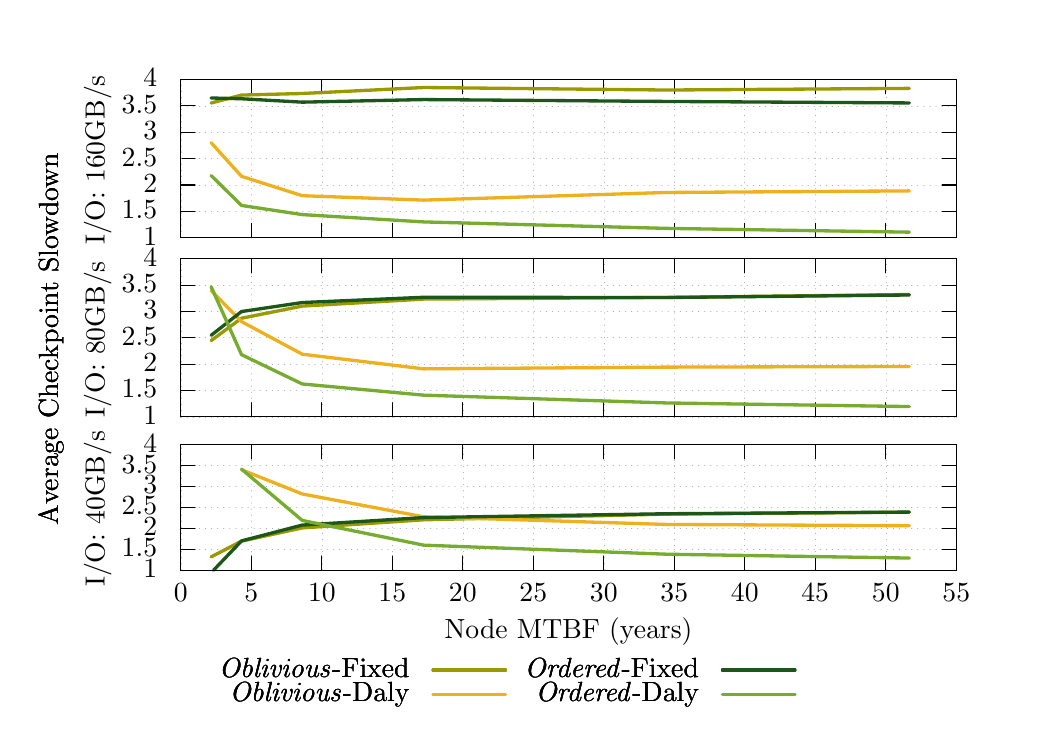
\begin{tikzpicture}[gnuplot]
%% generated with GNUPLOT 5.2p4 (Lua 5.3; terminal rev. 99 , script rev. 105)
%% Sat Sep 15 17:06:43 2018
\path (0.000,0.000) rectangle (12.500,8.750);
\gpcolor{color=gp lt color axes}
\gpsetlinetype{gp lt axes}
\gpsetdashtype{gp dt axes}
\gpsetlinewidth{0.50}
\draw[gp path] (1.945,1.860)--(11.793,1.860);
\gpcolor{color=gp lt color border}
\gpsetlinetype{gp lt border}
\gpsetdashtype{gp dt solid}
\gpsetlinewidth{1.00}
\draw[gp path] (1.945,1.860)--(2.125,1.860);
\draw[gp path] (11.793,1.860)--(11.613,1.860);
\node[gp node right] at (1.761,1.860) {$1$};
\gpcolor{color=gp lt color axes}
\gpsetlinetype{gp lt axes}
\gpsetdashtype{gp dt axes}
\gpsetlinewidth{0.50}
\draw[gp path] (1.945,2.126)--(11.793,2.126);
\gpcolor{color=gp lt color border}
\gpsetlinetype{gp lt border}
\gpsetdashtype{gp dt solid}
\gpsetlinewidth{1.00}
\draw[gp path] (1.945,2.126)--(2.125,2.126);
\draw[gp path] (11.793,2.126)--(11.613,2.126);
\node[gp node right] at (1.761,2.126) {$1.5$};
\gpcolor{color=gp lt color axes}
\gpsetlinetype{gp lt axes}
\gpsetdashtype{gp dt axes}
\gpsetlinewidth{0.50}
\draw[gp path] (1.945,2.391)--(11.793,2.391);
\gpcolor{color=gp lt color border}
\gpsetlinetype{gp lt border}
\gpsetdashtype{gp dt solid}
\gpsetlinewidth{1.00}
\draw[gp path] (1.945,2.391)--(2.125,2.391);
\draw[gp path] (11.793,2.391)--(11.613,2.391);
\node[gp node right] at (1.761,2.391) {$2$};
\gpcolor{color=gp lt color axes}
\gpsetlinetype{gp lt axes}
\gpsetdashtype{gp dt axes}
\gpsetlinewidth{0.50}
\draw[gp path] (1.945,2.657)--(11.793,2.657);
\gpcolor{color=gp lt color border}
\gpsetlinetype{gp lt border}
\gpsetdashtype{gp dt solid}
\gpsetlinewidth{1.00}
\draw[gp path] (1.945,2.657)--(2.125,2.657);
\draw[gp path] (11.793,2.657)--(11.613,2.657);
\node[gp node right] at (1.761,2.657) {$2.5$};
\gpcolor{color=gp lt color axes}
\gpsetlinetype{gp lt axes}
\gpsetdashtype{gp dt axes}
\gpsetlinewidth{0.50}
\draw[gp path] (1.945,2.923)--(11.793,2.923);
\gpcolor{color=gp lt color border}
\gpsetlinetype{gp lt border}
\gpsetdashtype{gp dt solid}
\gpsetlinewidth{1.00}
\draw[gp path] (1.945,2.923)--(2.125,2.923);
\draw[gp path] (11.793,2.923)--(11.613,2.923);
\node[gp node right] at (1.761,2.923) {$3$};
\gpcolor{color=gp lt color axes}
\gpsetlinetype{gp lt axes}
\gpsetdashtype{gp dt axes}
\gpsetlinewidth{0.50}
\draw[gp path] (1.945,3.188)--(11.793,3.188);
\gpcolor{color=gp lt color border}
\gpsetlinetype{gp lt border}
\gpsetdashtype{gp dt solid}
\gpsetlinewidth{1.00}
\draw[gp path] (1.945,3.188)--(2.125,3.188);
\draw[gp path] (11.793,3.188)--(11.613,3.188);
\node[gp node right] at (1.761,3.188) {$3.5$};
\gpcolor{color=gp lt color axes}
\gpsetlinetype{gp lt axes}
\gpsetdashtype{gp dt axes}
\gpsetlinewidth{0.50}
\draw[gp path] (1.945,3.454)--(11.793,3.454);
\gpcolor{color=gp lt color border}
\gpsetlinetype{gp lt border}
\gpsetdashtype{gp dt solid}
\gpsetlinewidth{1.00}
\draw[gp path] (1.945,3.454)--(2.125,3.454);
\draw[gp path] (11.793,3.454)--(11.613,3.454);
\node[gp node right] at (1.761,3.454) {$4$};
\gpcolor{color=gp lt color axes}
\gpsetlinetype{gp lt axes}
\gpsetdashtype{gp dt axes}
\gpsetlinewidth{0.50}
\draw[gp path] (1.945,1.860)--(1.945,3.454);
\gpcolor{color=gp lt color border}
\gpsetlinetype{gp lt border}
\gpsetdashtype{gp dt solid}
\gpsetlinewidth{1.00}
\draw[gp path] (1.945,1.860)--(1.945,2.040);
\draw[gp path] (1.945,3.454)--(1.945,3.274);
\node[gp node center] at (1.945,1.552) {$0$};
\gpcolor{color=gp lt color axes}
\gpsetlinetype{gp lt axes}
\gpsetdashtype{gp dt axes}
\gpsetlinewidth{0.50}
\draw[gp path] (2.840,1.860)--(2.840,3.454);
\gpcolor{color=gp lt color border}
\gpsetlinetype{gp lt border}
\gpsetdashtype{gp dt solid}
\gpsetlinewidth{1.00}
\draw[gp path] (2.840,1.860)--(2.840,2.040);
\draw[gp path] (2.840,3.454)--(2.840,3.274);
\node[gp node center] at (2.840,1.552) {$5$};
\gpcolor{color=gp lt color axes}
\gpsetlinetype{gp lt axes}
\gpsetdashtype{gp dt axes}
\gpsetlinewidth{0.50}
\draw[gp path] (3.736,1.860)--(3.736,3.454);
\gpcolor{color=gp lt color border}
\gpsetlinetype{gp lt border}
\gpsetdashtype{gp dt solid}
\gpsetlinewidth{1.00}
\draw[gp path] (3.736,1.860)--(3.736,2.040);
\draw[gp path] (3.736,3.454)--(3.736,3.274);
\node[gp node center] at (3.736,1.552) {$10$};
\gpcolor{color=gp lt color axes}
\gpsetlinetype{gp lt axes}
\gpsetdashtype{gp dt axes}
\gpsetlinewidth{0.50}
\draw[gp path] (4.631,1.860)--(4.631,3.454);
\gpcolor{color=gp lt color border}
\gpsetlinetype{gp lt border}
\gpsetdashtype{gp dt solid}
\gpsetlinewidth{1.00}
\draw[gp path] (4.631,1.860)--(4.631,2.040);
\draw[gp path] (4.631,3.454)--(4.631,3.274);
\node[gp node center] at (4.631,1.552) {$15$};
\gpcolor{color=gp lt color axes}
\gpsetlinetype{gp lt axes}
\gpsetdashtype{gp dt axes}
\gpsetlinewidth{0.50}
\draw[gp path] (5.526,1.860)--(5.526,3.454);
\gpcolor{color=gp lt color border}
\gpsetlinetype{gp lt border}
\gpsetdashtype{gp dt solid}
\gpsetlinewidth{1.00}
\draw[gp path] (5.526,1.860)--(5.526,2.040);
\draw[gp path] (5.526,3.454)--(5.526,3.274);
\node[gp node center] at (5.526,1.552) {$20$};
\gpcolor{color=gp lt color axes}
\gpsetlinetype{gp lt axes}
\gpsetdashtype{gp dt axes}
\gpsetlinewidth{0.50}
\draw[gp path] (6.421,1.860)--(6.421,3.454);
\gpcolor{color=gp lt color border}
\gpsetlinetype{gp lt border}
\gpsetdashtype{gp dt solid}
\gpsetlinewidth{1.00}
\draw[gp path] (6.421,1.860)--(6.421,2.040);
\draw[gp path] (6.421,3.454)--(6.421,3.274);
\node[gp node center] at (6.421,1.552) {$25$};
\gpcolor{color=gp lt color axes}
\gpsetlinetype{gp lt axes}
\gpsetdashtype{gp dt axes}
\gpsetlinewidth{0.50}
\draw[gp path] (7.317,1.860)--(7.317,3.454);
\gpcolor{color=gp lt color border}
\gpsetlinetype{gp lt border}
\gpsetdashtype{gp dt solid}
\gpsetlinewidth{1.00}
\draw[gp path] (7.317,1.860)--(7.317,2.040);
\draw[gp path] (7.317,3.454)--(7.317,3.274);
\node[gp node center] at (7.317,1.552) {$30$};
\gpcolor{color=gp lt color axes}
\gpsetlinetype{gp lt axes}
\gpsetdashtype{gp dt axes}
\gpsetlinewidth{0.50}
\draw[gp path] (8.212,1.860)--(8.212,3.454);
\gpcolor{color=gp lt color border}
\gpsetlinetype{gp lt border}
\gpsetdashtype{gp dt solid}
\gpsetlinewidth{1.00}
\draw[gp path] (8.212,1.860)--(8.212,2.040);
\draw[gp path] (8.212,3.454)--(8.212,3.274);
\node[gp node center] at (8.212,1.552) {$35$};
\gpcolor{color=gp lt color axes}
\gpsetlinetype{gp lt axes}
\gpsetdashtype{gp dt axes}
\gpsetlinewidth{0.50}
\draw[gp path] (9.107,1.860)--(9.107,3.454);
\gpcolor{color=gp lt color border}
\gpsetlinetype{gp lt border}
\gpsetdashtype{gp dt solid}
\gpsetlinewidth{1.00}
\draw[gp path] (9.107,1.860)--(9.107,2.040);
\draw[gp path] (9.107,3.454)--(9.107,3.274);
\node[gp node center] at (9.107,1.552) {$40$};
\gpcolor{color=gp lt color axes}
\gpsetlinetype{gp lt axes}
\gpsetdashtype{gp dt axes}
\gpsetlinewidth{0.50}
\draw[gp path] (10.002,1.860)--(10.002,3.454);
\gpcolor{color=gp lt color border}
\gpsetlinetype{gp lt border}
\gpsetdashtype{gp dt solid}
\gpsetlinewidth{1.00}
\draw[gp path] (10.002,1.860)--(10.002,2.040);
\draw[gp path] (10.002,3.454)--(10.002,3.274);
\node[gp node center] at (10.002,1.552) {$45$};
\gpcolor{color=gp lt color axes}
\gpsetlinetype{gp lt axes}
\gpsetdashtype{gp dt axes}
\gpsetlinewidth{0.50}
\draw[gp path] (10.898,1.860)--(10.898,3.454);
\gpcolor{color=gp lt color border}
\gpsetlinetype{gp lt border}
\gpsetdashtype{gp dt solid}
\gpsetlinewidth{1.00}
\draw[gp path] (10.898,1.860)--(10.898,2.040);
\draw[gp path] (10.898,3.454)--(10.898,3.274);
\node[gp node center] at (10.898,1.552) {$50$};
\gpcolor{color=gp lt color axes}
\gpsetlinetype{gp lt axes}
\gpsetdashtype{gp dt axes}
\gpsetlinewidth{0.50}
\draw[gp path] (11.793,1.860)--(11.793,3.454);
\gpcolor{color=gp lt color border}
\gpsetlinetype{gp lt border}
\gpsetdashtype{gp dt solid}
\gpsetlinewidth{1.00}
\draw[gp path] (11.793,1.860)--(11.793,2.040);
\draw[gp path] (11.793,3.454)--(11.793,3.274);
\node[gp node center] at (11.793,1.552) {$55$};
\draw[gp path] (1.945,3.454)--(1.945,1.860)--(11.793,1.860)--(11.793,3.454)--cycle;
\node[gp node center,rotate=90] at (0.312,4.812) {Average Checkpoint Slowdown};
\node[gp node center,rotate=-270] at (0.901,2.657) {I/O: 40GB/s};
\node[gp node center] at (6.869,1.090) {Node MTBF (years)};
\node[gp node right] at (4.966,0.591) {\propfixed};
\gpcolor{rgb color={0.604,0.600,0.000}}
\gpsetlinewidth{3.00}
\draw[gp path] (5.150,0.591)--(6.066,0.591);
\draw[gp path] (2.330,2.029)--(2.716,2.229)--(3.487,2.397)--(5.029,2.500)--(8.113,2.572)%
  --(11.197,2.597);
\gpcolor{color=gp lt color border}
\node[gp node right] at (4.966,0.283) {\propdaly};
\gpcolor{rgb color={0.929,0.694,0.125}}
\draw[gp path] (5.150,0.283)--(6.066,0.283);
\draw[gp path] (2.716,3.136)--(3.487,2.828)--(5.029,2.538)--(8.113,2.441)--(11.197,2.425);
\gpcolor{color=gp lt color border}
\node[gp node right] at (8.642,0.591) {\bfifofixed};
\gpcolor{rgb color={0.110,0.337,0.094}}
\draw[gp path] (8.826,0.591)--(9.742,0.591);
\draw[gp path] (2.361,1.860)--(2.716,2.232)--(3.487,2.433)--(5.029,2.528)--(8.113,2.577)%
  --(11.197,2.598);
\gpcolor{color=gp lt color border}
\node[gp node right] at (8.642,0.283) {\bfifodaly};
\gpcolor{rgb color={0.467,0.675,0.188}}
\draw[gp path] (8.826,0.283)--(9.742,0.283);
\draw[gp path] (2.716,3.144)--(3.487,2.492)--(5.029,2.178)--(8.113,2.063)--(11.197,2.014);
\gpcolor{color=gp lt color border}
\gpsetlinewidth{1.00}
\draw[gp path] (1.945,3.454)--(1.945,1.860)--(11.793,1.860)--(11.793,3.454)--cycle;
%% coordinates of the plot area
\gpdefrectangularnode{gp plot 1}{\pgfpoint{1.945cm}{1.860cm}}{\pgfpoint{11.793cm}{3.454cm}}
\gpcolor{color=gp lt color axes}
\gpsetlinetype{gp lt axes}
\gpsetdashtype{gp dt axes}
\gpsetlinewidth{0.50}
\draw[gp path] (1.945,3.808)--(11.793,3.808);
\gpcolor{color=gp lt color border}
\gpsetlinetype{gp lt border}
\gpsetdashtype{gp dt solid}
\gpsetlinewidth{1.00}
\draw[gp path] (1.945,3.808)--(2.125,3.808);
\draw[gp path] (11.793,3.808)--(11.613,3.808);
\node[gp node right] at (1.761,3.808) {$1$};
\gpcolor{color=gp lt color axes}
\gpsetlinetype{gp lt axes}
\gpsetdashtype{gp dt axes}
\gpsetlinewidth{0.50}
\draw[gp path] (1.945,4.143)--(11.793,4.143);
\gpcolor{color=gp lt color border}
\gpsetlinetype{gp lt border}
\gpsetdashtype{gp dt solid}
\gpsetlinewidth{1.00}
\draw[gp path] (1.945,4.143)--(2.125,4.143);
\draw[gp path] (11.793,4.143)--(11.613,4.143);
\node[gp node right] at (1.761,4.143) {$1.5$};
\gpcolor{color=gp lt color axes}
\gpsetlinetype{gp lt axes}
\gpsetdashtype{gp dt axes}
\gpsetlinewidth{0.50}
\draw[gp path] (1.945,4.477)--(11.793,4.477);
\gpcolor{color=gp lt color border}
\gpsetlinetype{gp lt border}
\gpsetdashtype{gp dt solid}
\gpsetlinewidth{1.00}
\draw[gp path] (1.945,4.477)--(2.125,4.477);
\draw[gp path] (11.793,4.477)--(11.613,4.477);
\node[gp node right] at (1.761,4.477) {$2$};
\gpcolor{color=gp lt color axes}
\gpsetlinetype{gp lt axes}
\gpsetdashtype{gp dt axes}
\gpsetlinewidth{0.50}
\draw[gp path] (1.945,4.812)--(11.793,4.812);
\gpcolor{color=gp lt color border}
\gpsetlinetype{gp lt border}
\gpsetdashtype{gp dt solid}
\gpsetlinewidth{1.00}
\draw[gp path] (1.945,4.812)--(2.125,4.812);
\draw[gp path] (11.793,4.812)--(11.613,4.812);
\node[gp node right] at (1.761,4.812) {$2.5$};
\gpcolor{color=gp lt color axes}
\gpsetlinetype{gp lt axes}
\gpsetdashtype{gp dt axes}
\gpsetlinewidth{0.50}
\draw[gp path] (1.945,5.147)--(11.793,5.147);
\gpcolor{color=gp lt color border}
\gpsetlinetype{gp lt border}
\gpsetdashtype{gp dt solid}
\gpsetlinewidth{1.00}
\draw[gp path] (1.945,5.147)--(2.125,5.147);
\draw[gp path] (11.793,5.147)--(11.613,5.147);
\node[gp node right] at (1.761,5.147) {$3$};
\gpcolor{color=gp lt color axes}
\gpsetlinetype{gp lt axes}
\gpsetdashtype{gp dt axes}
\gpsetlinewidth{0.50}
\draw[gp path] (1.945,5.481)--(11.793,5.481);
\gpcolor{color=gp lt color border}
\gpsetlinetype{gp lt border}
\gpsetdashtype{gp dt solid}
\gpsetlinewidth{1.00}
\draw[gp path] (1.945,5.481)--(2.125,5.481);
\draw[gp path] (11.793,5.481)--(11.613,5.481);
\node[gp node right] at (1.761,5.481) {$3.5$};
\gpcolor{color=gp lt color axes}
\gpsetlinetype{gp lt axes}
\gpsetdashtype{gp dt axes}
\gpsetlinewidth{0.50}
\draw[gp path] (1.945,5.816)--(11.793,5.816);
\gpcolor{color=gp lt color border}
\gpsetlinetype{gp lt border}
\gpsetdashtype{gp dt solid}
\gpsetlinewidth{1.00}
\draw[gp path] (1.945,5.816)--(2.125,5.816);
\draw[gp path] (11.793,5.816)--(11.613,5.816);
\node[gp node right] at (1.761,5.816) {$4$};
\gpcolor{color=gp lt color axes}
\gpsetlinetype{gp lt axes}
\gpsetdashtype{gp dt axes}
\gpsetlinewidth{0.50}
\draw[gp path] (1.945,3.808)--(1.945,5.816);
\gpcolor{color=gp lt color border}
\gpsetlinetype{gp lt border}
\gpsetdashtype{gp dt solid}
\gpsetlinewidth{1.00}
\draw[gp path] (1.945,3.808)--(1.945,3.988);
\draw[gp path] (1.945,5.816)--(1.945,5.636);
\gpcolor{color=gp lt color axes}
\gpsetlinetype{gp lt axes}
\gpsetdashtype{gp dt axes}
\gpsetlinewidth{0.50}
\draw[gp path] (2.840,3.808)--(2.840,5.816);
\gpcolor{color=gp lt color border}
\gpsetlinetype{gp lt border}
\gpsetdashtype{gp dt solid}
\gpsetlinewidth{1.00}
\draw[gp path] (2.840,3.808)--(2.840,3.988);
\draw[gp path] (2.840,5.816)--(2.840,5.636);
\gpcolor{color=gp lt color axes}
\gpsetlinetype{gp lt axes}
\gpsetdashtype{gp dt axes}
\gpsetlinewidth{0.50}
\draw[gp path] (3.736,3.808)--(3.736,5.816);
\gpcolor{color=gp lt color border}
\gpsetlinetype{gp lt border}
\gpsetdashtype{gp dt solid}
\gpsetlinewidth{1.00}
\draw[gp path] (3.736,3.808)--(3.736,3.988);
\draw[gp path] (3.736,5.816)--(3.736,5.636);
\gpcolor{color=gp lt color axes}
\gpsetlinetype{gp lt axes}
\gpsetdashtype{gp dt axes}
\gpsetlinewidth{0.50}
\draw[gp path] (4.631,3.808)--(4.631,5.816);
\gpcolor{color=gp lt color border}
\gpsetlinetype{gp lt border}
\gpsetdashtype{gp dt solid}
\gpsetlinewidth{1.00}
\draw[gp path] (4.631,3.808)--(4.631,3.988);
\draw[gp path] (4.631,5.816)--(4.631,5.636);
\gpcolor{color=gp lt color axes}
\gpsetlinetype{gp lt axes}
\gpsetdashtype{gp dt axes}
\gpsetlinewidth{0.50}
\draw[gp path] (5.526,3.808)--(5.526,5.816);
\gpcolor{color=gp lt color border}
\gpsetlinetype{gp lt border}
\gpsetdashtype{gp dt solid}
\gpsetlinewidth{1.00}
\draw[gp path] (5.526,3.808)--(5.526,3.988);
\draw[gp path] (5.526,5.816)--(5.526,5.636);
\gpcolor{color=gp lt color axes}
\gpsetlinetype{gp lt axes}
\gpsetdashtype{gp dt axes}
\gpsetlinewidth{0.50}
\draw[gp path] (6.421,3.808)--(6.421,5.816);
\gpcolor{color=gp lt color border}
\gpsetlinetype{gp lt border}
\gpsetdashtype{gp dt solid}
\gpsetlinewidth{1.00}
\draw[gp path] (6.421,3.808)--(6.421,3.988);
\draw[gp path] (6.421,5.816)--(6.421,5.636);
\gpcolor{color=gp lt color axes}
\gpsetlinetype{gp lt axes}
\gpsetdashtype{gp dt axes}
\gpsetlinewidth{0.50}
\draw[gp path] (7.317,3.808)--(7.317,5.816);
\gpcolor{color=gp lt color border}
\gpsetlinetype{gp lt border}
\gpsetdashtype{gp dt solid}
\gpsetlinewidth{1.00}
\draw[gp path] (7.317,3.808)--(7.317,3.988);
\draw[gp path] (7.317,5.816)--(7.317,5.636);
\gpcolor{color=gp lt color axes}
\gpsetlinetype{gp lt axes}
\gpsetdashtype{gp dt axes}
\gpsetlinewidth{0.50}
\draw[gp path] (8.212,3.808)--(8.212,5.816);
\gpcolor{color=gp lt color border}
\gpsetlinetype{gp lt border}
\gpsetdashtype{gp dt solid}
\gpsetlinewidth{1.00}
\draw[gp path] (8.212,3.808)--(8.212,3.988);
\draw[gp path] (8.212,5.816)--(8.212,5.636);
\gpcolor{color=gp lt color axes}
\gpsetlinetype{gp lt axes}
\gpsetdashtype{gp dt axes}
\gpsetlinewidth{0.50}
\draw[gp path] (9.107,3.808)--(9.107,5.816);
\gpcolor{color=gp lt color border}
\gpsetlinetype{gp lt border}
\gpsetdashtype{gp dt solid}
\gpsetlinewidth{1.00}
\draw[gp path] (9.107,3.808)--(9.107,3.988);
\draw[gp path] (9.107,5.816)--(9.107,5.636);
\gpcolor{color=gp lt color axes}
\gpsetlinetype{gp lt axes}
\gpsetdashtype{gp dt axes}
\gpsetlinewidth{0.50}
\draw[gp path] (10.002,3.808)--(10.002,5.816);
\gpcolor{color=gp lt color border}
\gpsetlinetype{gp lt border}
\gpsetdashtype{gp dt solid}
\gpsetlinewidth{1.00}
\draw[gp path] (10.002,3.808)--(10.002,3.988);
\draw[gp path] (10.002,5.816)--(10.002,5.636);
\gpcolor{color=gp lt color axes}
\gpsetlinetype{gp lt axes}
\gpsetdashtype{gp dt axes}
\gpsetlinewidth{0.50}
\draw[gp path] (10.898,3.808)--(10.898,5.816);
\gpcolor{color=gp lt color border}
\gpsetlinetype{gp lt border}
\gpsetdashtype{gp dt solid}
\gpsetlinewidth{1.00}
\draw[gp path] (10.898,3.808)--(10.898,3.988);
\draw[gp path] (10.898,5.816)--(10.898,5.636);
\gpcolor{color=gp lt color axes}
\gpsetlinetype{gp lt axes}
\gpsetdashtype{gp dt axes}
\gpsetlinewidth{0.50}
\draw[gp path] (11.793,3.808)--(11.793,5.816);
\gpcolor{color=gp lt color border}
\gpsetlinetype{gp lt border}
\gpsetdashtype{gp dt solid}
\gpsetlinewidth{1.00}
\draw[gp path] (11.793,3.808)--(11.793,3.988);
\draw[gp path] (11.793,5.816)--(11.793,5.636);
\draw[gp path] (1.945,5.816)--(1.945,3.808)--(11.793,3.808)--(11.793,5.816)--cycle;
\node[gp node center,rotate=90] at (0.312,4.812) {Average Checkpoint Slowdown};
\node[gp node center,rotate=-270] at (0.901,4.812) {I/O: 80GB/s};
\node[gp node right] at (4.966,0.591) {\propfixed};
\gpcolor{rgb color={0.604,0.600,0.000}}
\gpsetlinewidth{3.00}
\draw[gp path] (5.150,0.591)--(6.066,0.591);
\draw[gp path] (2.330,4.776)--(2.716,5.060)--(3.487,5.214)--(5.029,5.303)--(8.113,5.324)%
  --(11.197,5.361);
\gpcolor{color=gp lt color border}
\node[gp node right] at (4.966,0.283) {\propdaly};
\gpcolor{rgb color={0.929,0.694,0.125}}
\draw[gp path] (5.150,0.283)--(6.066,0.283);
\draw[gp path] (2.330,5.412)--(2.716,5.017)--(3.487,4.603)--(5.029,4.417)--(8.113,4.439)%
  --(11.197,4.447);
\gpcolor{color=gp lt color border}
\node[gp node right] at (8.642,0.591) {\bfifofixed};
\gpcolor{rgb color={0.110,0.337,0.094}}
\draw[gp path] (8.826,0.591)--(9.742,0.591);
\draw[gp path] (2.330,4.843)--(2.716,5.145)--(3.487,5.259)--(5.029,5.326)--(8.113,5.323)%
  --(11.197,5.355);
\gpcolor{color=gp lt color border}
\node[gp node right] at (8.642,0.283) {\bfifodaly};
\gpcolor{rgb color={0.467,0.675,0.188}}
\draw[gp path] (8.826,0.283)--(9.742,0.283);
\draw[gp path] (2.330,5.460)--(2.716,4.597)--(3.487,4.225)--(5.029,4.083)--(8.113,3.984)%
  --(11.197,3.938);
\gpcolor{color=gp lt color border}
\gpsetlinewidth{1.00}
\draw[gp path] (1.945,5.816)--(1.945,3.808)--(11.793,3.808)--(11.793,5.816)--cycle;
%% coordinates of the plot area
\gpdefrectangularnode{gp plot 2}{\pgfpoint{1.945cm}{3.808cm}}{\pgfpoint{11.793cm}{5.816cm}}
\gpcolor{color=gp lt color axes}
\gpsetlinetype{gp lt axes}
\gpsetdashtype{gp dt axes}
\gpsetlinewidth{0.50}
\draw[gp path] (1.945,6.083)--(11.793,6.083);
\gpcolor{color=gp lt color border}
\gpsetlinetype{gp lt border}
\gpsetdashtype{gp dt solid}
\gpsetlinewidth{1.00}
\draw[gp path] (1.945,6.083)--(2.125,6.083);
\draw[gp path] (11.793,6.083)--(11.613,6.083);
\node[gp node right] at (1.761,6.083) {$1$};
\gpcolor{color=gp lt color axes}
\gpsetlinetype{gp lt axes}
\gpsetdashtype{gp dt axes}
\gpsetlinewidth{0.50}
\draw[gp path] (1.945,6.418)--(11.793,6.418);
\gpcolor{color=gp lt color border}
\gpsetlinetype{gp lt border}
\gpsetdashtype{gp dt solid}
\gpsetlinewidth{1.00}
\draw[gp path] (1.945,6.418)--(2.125,6.418);
\draw[gp path] (11.793,6.418)--(11.613,6.418);
\node[gp node right] at (1.761,6.418) {$1.5$};
\gpcolor{color=gp lt color axes}
\gpsetlinetype{gp lt axes}
\gpsetdashtype{gp dt axes}
\gpsetlinewidth{0.50}
\draw[gp path] (1.945,6.752)--(11.793,6.752);
\gpcolor{color=gp lt color border}
\gpsetlinetype{gp lt border}
\gpsetdashtype{gp dt solid}
\gpsetlinewidth{1.00}
\draw[gp path] (1.945,6.752)--(2.125,6.752);
\draw[gp path] (11.793,6.752)--(11.613,6.752);
\node[gp node right] at (1.761,6.752) {$2$};
\gpcolor{color=gp lt color axes}
\gpsetlinetype{gp lt axes}
\gpsetdashtype{gp dt axes}
\gpsetlinewidth{0.50}
\draw[gp path] (1.945,7.087)--(11.793,7.087);
\gpcolor{color=gp lt color border}
\gpsetlinetype{gp lt border}
\gpsetdashtype{gp dt solid}
\gpsetlinewidth{1.00}
\draw[gp path] (1.945,7.087)--(2.125,7.087);
\draw[gp path] (11.793,7.087)--(11.613,7.087);
\node[gp node right] at (1.761,7.087) {$2.5$};
\gpcolor{color=gp lt color axes}
\gpsetlinetype{gp lt axes}
\gpsetdashtype{gp dt axes}
\gpsetlinewidth{0.50}
\draw[gp path] (1.945,7.422)--(11.793,7.422);
\gpcolor{color=gp lt color border}
\gpsetlinetype{gp lt border}
\gpsetdashtype{gp dt solid}
\gpsetlinewidth{1.00}
\draw[gp path] (1.945,7.422)--(2.125,7.422);
\draw[gp path] (11.793,7.422)--(11.613,7.422);
\node[gp node right] at (1.761,7.422) {$3$};
\gpcolor{color=gp lt color axes}
\gpsetlinetype{gp lt axes}
\gpsetdashtype{gp dt axes}
\gpsetlinewidth{0.50}
\draw[gp path] (1.945,7.756)--(11.793,7.756);
\gpcolor{color=gp lt color border}
\gpsetlinetype{gp lt border}
\gpsetdashtype{gp dt solid}
\gpsetlinewidth{1.00}
\draw[gp path] (1.945,7.756)--(2.125,7.756);
\draw[gp path] (11.793,7.756)--(11.613,7.756);
\node[gp node right] at (1.761,7.756) {$3.5$};
\gpcolor{color=gp lt color axes}
\gpsetlinetype{gp lt axes}
\gpsetdashtype{gp dt axes}
\gpsetlinewidth{0.50}
\draw[gp path] (1.945,8.091)--(11.793,8.091);
\gpcolor{color=gp lt color border}
\gpsetlinetype{gp lt border}
\gpsetdashtype{gp dt solid}
\gpsetlinewidth{1.00}
\draw[gp path] (1.945,8.091)--(2.125,8.091);
\draw[gp path] (11.793,8.091)--(11.613,8.091);
\node[gp node right] at (1.761,8.091) {$4$};
\gpcolor{color=gp lt color axes}
\gpsetlinetype{gp lt axes}
\gpsetdashtype{gp dt axes}
\gpsetlinewidth{0.50}
\draw[gp path] (1.945,6.083)--(1.945,8.091);
\gpcolor{color=gp lt color border}
\gpsetlinetype{gp lt border}
\gpsetdashtype{gp dt solid}
\gpsetlinewidth{1.00}
\draw[gp path] (1.945,6.083)--(1.945,6.263);
\draw[gp path] (1.945,8.091)--(1.945,7.911);
\gpcolor{color=gp lt color axes}
\gpsetlinetype{gp lt axes}
\gpsetdashtype{gp dt axes}
\gpsetlinewidth{0.50}
\draw[gp path] (2.840,6.083)--(2.840,8.091);
\gpcolor{color=gp lt color border}
\gpsetlinetype{gp lt border}
\gpsetdashtype{gp dt solid}
\gpsetlinewidth{1.00}
\draw[gp path] (2.840,6.083)--(2.840,6.263);
\draw[gp path] (2.840,8.091)--(2.840,7.911);
\gpcolor{color=gp lt color axes}
\gpsetlinetype{gp lt axes}
\gpsetdashtype{gp dt axes}
\gpsetlinewidth{0.50}
\draw[gp path] (3.736,6.083)--(3.736,8.091);
\gpcolor{color=gp lt color border}
\gpsetlinetype{gp lt border}
\gpsetdashtype{gp dt solid}
\gpsetlinewidth{1.00}
\draw[gp path] (3.736,6.083)--(3.736,6.263);
\draw[gp path] (3.736,8.091)--(3.736,7.911);
\gpcolor{color=gp lt color axes}
\gpsetlinetype{gp lt axes}
\gpsetdashtype{gp dt axes}
\gpsetlinewidth{0.50}
\draw[gp path] (4.631,6.083)--(4.631,8.091);
\gpcolor{color=gp lt color border}
\gpsetlinetype{gp lt border}
\gpsetdashtype{gp dt solid}
\gpsetlinewidth{1.00}
\draw[gp path] (4.631,6.083)--(4.631,6.263);
\draw[gp path] (4.631,8.091)--(4.631,7.911);
\gpcolor{color=gp lt color axes}
\gpsetlinetype{gp lt axes}
\gpsetdashtype{gp dt axes}
\gpsetlinewidth{0.50}
\draw[gp path] (5.526,6.083)--(5.526,8.091);
\gpcolor{color=gp lt color border}
\gpsetlinetype{gp lt border}
\gpsetdashtype{gp dt solid}
\gpsetlinewidth{1.00}
\draw[gp path] (5.526,6.083)--(5.526,6.263);
\draw[gp path] (5.526,8.091)--(5.526,7.911);
\gpcolor{color=gp lt color axes}
\gpsetlinetype{gp lt axes}
\gpsetdashtype{gp dt axes}
\gpsetlinewidth{0.50}
\draw[gp path] (6.421,6.083)--(6.421,8.091);
\gpcolor{color=gp lt color border}
\gpsetlinetype{gp lt border}
\gpsetdashtype{gp dt solid}
\gpsetlinewidth{1.00}
\draw[gp path] (6.421,6.083)--(6.421,6.263);
\draw[gp path] (6.421,8.091)--(6.421,7.911);
\gpcolor{color=gp lt color axes}
\gpsetlinetype{gp lt axes}
\gpsetdashtype{gp dt axes}
\gpsetlinewidth{0.50}
\draw[gp path] (7.317,6.083)--(7.317,8.091);
\gpcolor{color=gp lt color border}
\gpsetlinetype{gp lt border}
\gpsetdashtype{gp dt solid}
\gpsetlinewidth{1.00}
\draw[gp path] (7.317,6.083)--(7.317,6.263);
\draw[gp path] (7.317,8.091)--(7.317,7.911);
\gpcolor{color=gp lt color axes}
\gpsetlinetype{gp lt axes}
\gpsetdashtype{gp dt axes}
\gpsetlinewidth{0.50}
\draw[gp path] (8.212,6.083)--(8.212,8.091);
\gpcolor{color=gp lt color border}
\gpsetlinetype{gp lt border}
\gpsetdashtype{gp dt solid}
\gpsetlinewidth{1.00}
\draw[gp path] (8.212,6.083)--(8.212,6.263);
\draw[gp path] (8.212,8.091)--(8.212,7.911);
\gpcolor{color=gp lt color axes}
\gpsetlinetype{gp lt axes}
\gpsetdashtype{gp dt axes}
\gpsetlinewidth{0.50}
\draw[gp path] (9.107,6.083)--(9.107,8.091);
\gpcolor{color=gp lt color border}
\gpsetlinetype{gp lt border}
\gpsetdashtype{gp dt solid}
\gpsetlinewidth{1.00}
\draw[gp path] (9.107,6.083)--(9.107,6.263);
\draw[gp path] (9.107,8.091)--(9.107,7.911);
\gpcolor{color=gp lt color axes}
\gpsetlinetype{gp lt axes}
\gpsetdashtype{gp dt axes}
\gpsetlinewidth{0.50}
\draw[gp path] (10.002,6.083)--(10.002,8.091);
\gpcolor{color=gp lt color border}
\gpsetlinetype{gp lt border}
\gpsetdashtype{gp dt solid}
\gpsetlinewidth{1.00}
\draw[gp path] (10.002,6.083)--(10.002,6.263);
\draw[gp path] (10.002,8.091)--(10.002,7.911);
\gpcolor{color=gp lt color axes}
\gpsetlinetype{gp lt axes}
\gpsetdashtype{gp dt axes}
\gpsetlinewidth{0.50}
\draw[gp path] (10.898,6.083)--(10.898,8.091);
\gpcolor{color=gp lt color border}
\gpsetlinetype{gp lt border}
\gpsetdashtype{gp dt solid}
\gpsetlinewidth{1.00}
\draw[gp path] (10.898,6.083)--(10.898,6.263);
\draw[gp path] (10.898,8.091)--(10.898,7.911);
\gpcolor{color=gp lt color axes}
\gpsetlinetype{gp lt axes}
\gpsetdashtype{gp dt axes}
\gpsetlinewidth{0.50}
\draw[gp path] (11.793,6.083)--(11.793,8.091);
\gpcolor{color=gp lt color border}
\gpsetlinetype{gp lt border}
\gpsetdashtype{gp dt solid}
\gpsetlinewidth{1.00}
\draw[gp path] (11.793,6.083)--(11.793,6.263);
\draw[gp path] (11.793,8.091)--(11.793,7.911);
\draw[gp path] (1.945,8.091)--(1.945,6.083)--(11.793,6.083)--(11.793,8.091)--cycle;
\node[gp node center,rotate=90] at (0.312,4.812) {Average Checkpoint Slowdown};
\node[gp node center,rotate=-270] at (0.901,7.087) {I/O: 160GB/s};
\node[gp node right] at (4.966,0.591) {\propfixed};
\gpcolor{rgb color={0.604,0.600,0.000}}
\gpsetlinewidth{3.00}
\draw[gp path] (5.150,0.591)--(6.066,0.591);
\draw[gp path] (2.330,7.793)--(2.716,7.894)--(3.487,7.914)--(5.029,7.990)--(8.113,7.958)%
  --(11.197,7.979);
\gpcolor{color=gp lt color border}
\node[gp node right] at (4.966,0.283) {\propdaly};
\gpcolor{rgb color={0.929,0.694,0.125}}
\draw[gp path] (5.150,0.283)--(6.066,0.283);
\draw[gp path] (2.330,7.289)--(2.716,6.862)--(3.487,6.616)--(5.029,6.560)--(8.113,6.657)%
  --(11.197,6.677);
\gpcolor{color=gp lt color border}
\node[gp node right] at (8.642,0.591) {\bfifofixed};
\gpcolor{rgb color={0.110,0.337,0.094}}
\draw[gp path] (8.826,0.591)--(9.742,0.591);
\draw[gp path] (2.330,7.857)--(2.716,7.847)--(3.487,7.804)--(5.029,7.837)--(8.113,7.813)%
  --(11.197,7.794);
\gpcolor{color=gp lt color border}
\node[gp node right] at (8.642,0.283) {\bfifodaly};
\gpcolor{rgb color={0.467,0.675,0.188}}
\draw[gp path] (8.826,0.283)--(9.742,0.283);
\draw[gp path] (2.330,6.872)--(2.716,6.492)--(3.487,6.376)--(5.029,6.283)--(8.113,6.201)%
  --(11.197,6.153);
\gpcolor{color=gp lt color border}
\gpsetlinewidth{1.00}
\draw[gp path] (1.945,8.091)--(1.945,6.083)--(11.793,6.083)--(11.793,8.091)--cycle;
%% coordinates of the plot area
\gpdefrectangularnode{gp plot 3}{\pgfpoint{1.945cm}{6.083cm}}{\pgfpoint{11.793cm}{8.091cm}}
\end{tikzpicture}
%% gnuplot variables
}
 \end{center}
      
      \end{frame}
      
      
      \begin{frame}
  \frametitle{Waste as a function of system bandwidth}
 
  \begin{center}
    \resizebox{0.95\linewidth}{!}{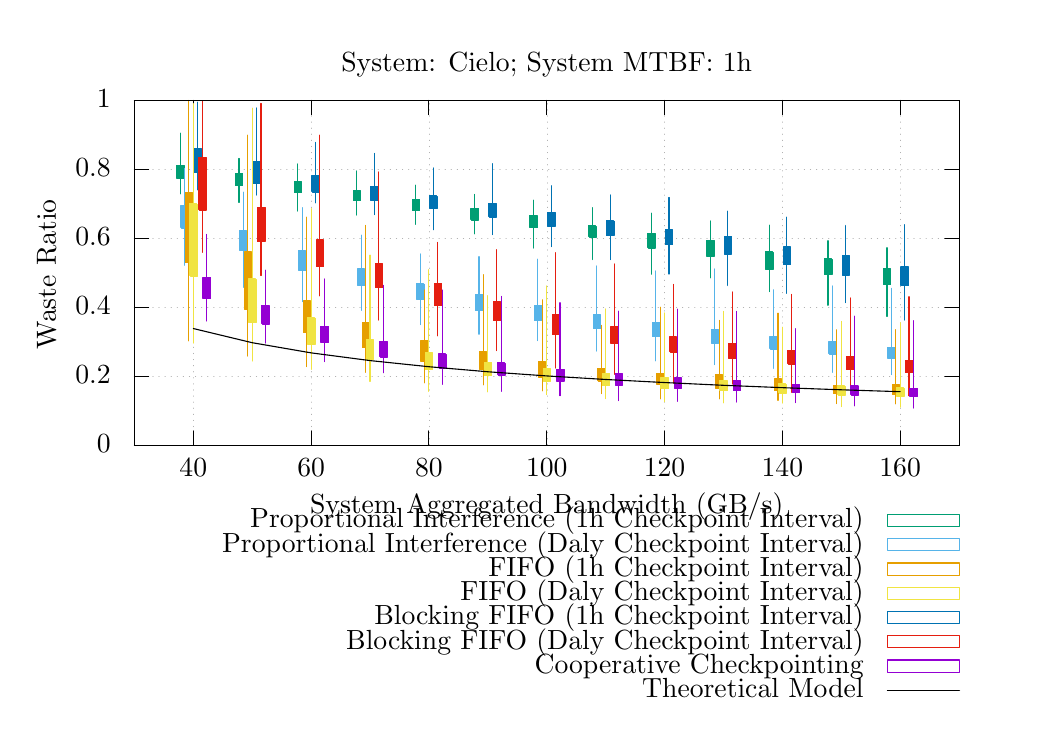
\begin{tikzpicture}[gnuplot]
%% generated with GNUPLOT 5.0p6 (Lua 5.3; terminal rev. 99, script rev. 100)
%% Wed Oct 18 12:28:52 2017
\path (0.000,0.000) rectangle (12.500,8.750);
\gpcolor{color=gp lt color axes}
\gpsetlinetype{gp lt axes}
\gpsetdashtype{gp dt axes}
\gpsetlinewidth{0.50}
\draw[gp path] (1.320,3.449)--(11.793,3.449);
\gpcolor{color=gp lt color border}
\gpsetlinetype{gp lt border}
\gpsetdashtype{gp dt solid}
\gpsetlinewidth{1.00}
\draw[gp path] (1.320,3.449)--(1.500,3.449);
\draw[gp path] (11.793,3.449)--(11.613,3.449);
\node[gp node right] at (1.136,3.449) {$0$};
\gpcolor{color=gp lt color axes}
\gpsetlinetype{gp lt axes}
\gpsetdashtype{gp dt axes}
\gpsetlinewidth{0.50}
\draw[gp path] (1.320,4.324)--(11.793,4.324);
\gpcolor{color=gp lt color border}
\gpsetlinetype{gp lt border}
\gpsetdashtype{gp dt solid}
\gpsetlinewidth{1.00}
\draw[gp path] (1.320,4.324)--(1.500,4.324);
\draw[gp path] (11.793,4.324)--(11.613,4.324);
\node[gp node right] at (1.136,4.324) {$0.2$};
\gpcolor{color=gp lt color axes}
\gpsetlinetype{gp lt axes}
\gpsetdashtype{gp dt axes}
\gpsetlinewidth{0.50}
\draw[gp path] (1.320,5.199)--(11.793,5.199);
\gpcolor{color=gp lt color border}
\gpsetlinetype{gp lt border}
\gpsetdashtype{gp dt solid}
\gpsetlinewidth{1.00}
\draw[gp path] (1.320,5.199)--(1.500,5.199);
\draw[gp path] (11.793,5.199)--(11.613,5.199);
\node[gp node right] at (1.136,5.199) {$0.4$};
\gpcolor{color=gp lt color axes}
\gpsetlinetype{gp lt axes}
\gpsetdashtype{gp dt axes}
\gpsetlinewidth{0.50}
\draw[gp path] (1.320,6.075)--(11.793,6.075);
\gpcolor{color=gp lt color border}
\gpsetlinetype{gp lt border}
\gpsetdashtype{gp dt solid}
\gpsetlinewidth{1.00}
\draw[gp path] (1.320,6.075)--(1.500,6.075);
\draw[gp path] (11.793,6.075)--(11.613,6.075);
\node[gp node right] at (1.136,6.075) {$0.6$};
\gpcolor{color=gp lt color axes}
\gpsetlinetype{gp lt axes}
\gpsetdashtype{gp dt axes}
\gpsetlinewidth{0.50}
\draw[gp path] (1.320,6.950)--(11.793,6.950);
\gpcolor{color=gp lt color border}
\gpsetlinetype{gp lt border}
\gpsetdashtype{gp dt solid}
\gpsetlinewidth{1.00}
\draw[gp path] (1.320,6.950)--(1.500,6.950);
\draw[gp path] (11.793,6.950)--(11.613,6.950);
\node[gp node right] at (1.136,6.950) {$0.8$};
\gpcolor{color=gp lt color axes}
\gpsetlinetype{gp lt axes}
\gpsetdashtype{gp dt axes}
\gpsetlinewidth{0.50}
\draw[gp path] (1.320,7.825)--(11.793,7.825);
\gpcolor{color=gp lt color border}
\gpsetlinetype{gp lt border}
\gpsetdashtype{gp dt solid}
\gpsetlinewidth{1.00}
\draw[gp path] (1.320,7.825)--(1.500,7.825);
\draw[gp path] (11.793,7.825)--(11.613,7.825);
\node[gp node right] at (1.136,7.825) {$1$};
\gpcolor{color=gp lt color axes}
\gpsetlinetype{gp lt axes}
\gpsetdashtype{gp dt axes}
\gpsetlinewidth{0.50}
\draw[gp path] (2.068,3.449)--(2.068,7.825);
\gpcolor{color=gp lt color border}
\gpsetlinetype{gp lt border}
\gpsetdashtype{gp dt solid}
\gpsetlinewidth{1.00}
\draw[gp path] (2.068,3.449)--(2.068,3.629);
\draw[gp path] (2.068,7.825)--(2.068,7.645);
\node[gp node center] at (2.068,3.141) {$40$};
\gpcolor{color=gp lt color axes}
\gpsetlinetype{gp lt axes}
\gpsetdashtype{gp dt axes}
\gpsetlinewidth{0.50}
\draw[gp path] (3.564,3.449)--(3.564,7.825);
\gpcolor{color=gp lt color border}
\gpsetlinetype{gp lt border}
\gpsetdashtype{gp dt solid}
\gpsetlinewidth{1.00}
\draw[gp path] (3.564,3.449)--(3.564,3.629);
\draw[gp path] (3.564,7.825)--(3.564,7.645);
\node[gp node center] at (3.564,3.141) {$60$};
\gpcolor{color=gp lt color axes}
\gpsetlinetype{gp lt axes}
\gpsetdashtype{gp dt axes}
\gpsetlinewidth{0.50}
\draw[gp path] (5.060,3.449)--(5.060,7.825);
\gpcolor{color=gp lt color border}
\gpsetlinetype{gp lt border}
\gpsetdashtype{gp dt solid}
\gpsetlinewidth{1.00}
\draw[gp path] (5.060,3.449)--(5.060,3.629);
\draw[gp path] (5.060,7.825)--(5.060,7.645);
\node[gp node center] at (5.060,3.141) {$80$};
\gpcolor{color=gp lt color axes}
\gpsetlinetype{gp lt axes}
\gpsetdashtype{gp dt axes}
\gpsetlinewidth{0.50}
\draw[gp path] (6.557,3.449)--(6.557,7.825);
\gpcolor{color=gp lt color border}
\gpsetlinetype{gp lt border}
\gpsetdashtype{gp dt solid}
\gpsetlinewidth{1.00}
\draw[gp path] (6.557,3.449)--(6.557,3.629);
\draw[gp path] (6.557,7.825)--(6.557,7.645);
\node[gp node center] at (6.557,3.141) {$100$};
\gpcolor{color=gp lt color axes}
\gpsetlinetype{gp lt axes}
\gpsetdashtype{gp dt axes}
\gpsetlinewidth{0.50}
\draw[gp path] (8.053,3.449)--(8.053,7.825);
\gpcolor{color=gp lt color border}
\gpsetlinetype{gp lt border}
\gpsetdashtype{gp dt solid}
\gpsetlinewidth{1.00}
\draw[gp path] (8.053,3.449)--(8.053,3.629);
\draw[gp path] (8.053,7.825)--(8.053,7.645);
\node[gp node center] at (8.053,3.141) {$120$};
\gpcolor{color=gp lt color axes}
\gpsetlinetype{gp lt axes}
\gpsetdashtype{gp dt axes}
\gpsetlinewidth{0.50}
\draw[gp path] (9.549,3.449)--(9.549,7.825);
\gpcolor{color=gp lt color border}
\gpsetlinetype{gp lt border}
\gpsetdashtype{gp dt solid}
\gpsetlinewidth{1.00}
\draw[gp path] (9.549,3.449)--(9.549,3.629);
\draw[gp path] (9.549,7.825)--(9.549,7.645);
\node[gp node center] at (9.549,3.141) {$140$};
\gpcolor{color=gp lt color axes}
\gpsetlinetype{gp lt axes}
\gpsetdashtype{gp dt axes}
\gpsetlinewidth{0.50}
\draw[gp path] (11.045,3.449)--(11.045,7.825);
\gpcolor{color=gp lt color border}
\gpsetlinetype{gp lt border}
\gpsetdashtype{gp dt solid}
\gpsetlinewidth{1.00}
\draw[gp path] (11.045,3.449)--(11.045,3.629);
\draw[gp path] (11.045,7.825)--(11.045,7.645);
\node[gp node center] at (11.045,3.141) {$160$};
\draw[gp path] (1.320,7.825)--(1.320,3.449)--(11.793,3.449)--(11.793,7.825)--cycle;
\node[gp node center,rotate=-270] at (0.246,5.637) {Waste Ratio};
\node[gp node center] at (6.556,2.679) {System Aggregated Bandwidth (GB/s)};
\node[gp node center] at (6.556,8.287) {System: Cielo; System MTBF: 1h};
\node[gp node right] at (10.698,2.490) {Proportional Interference (1h Checkpoint Interval)};
\gpcolor{rgb color={0.000,0.620,0.451}}
\draw[gp path] (10.882,2.413)--(11.798,2.413)--(11.798,2.567)--(10.882,2.567)--cycle;
\gpfill{rgb color={0.000,0.620,0.451}} (1.855,6.846)--(1.945,6.846)--(1.945,7.004)--(1.855,7.004)--cycle;
\draw[gp path] (1.900,6.639)--(1.900,6.846);
\draw[gp path] (1.900,7.004)--(1.900,7.409);
\draw[gp path] (1.855,7.004)--(1.945,7.004)--(1.945,6.846)--(1.855,6.846)--cycle;
\gpfill{rgb color={0.000,0.620,0.451}} (2.603,6.745)--(2.693,6.745)--(2.693,6.898)--(2.603,6.898)--cycle;
\draw[gp path] (2.648,6.531)--(2.648,6.745);
\draw[gp path] (2.648,6.898)--(2.648,7.089);
\draw[gp path] (2.603,6.898)--(2.693,6.898)--(2.693,6.745)--(2.603,6.745)--cycle;
\gpfill{rgb color={0.000,0.620,0.451}} (3.351,6.658)--(3.441,6.658)--(3.441,6.795)--(3.351,6.795)--cycle;
\draw[gp path] (3.396,6.420)--(3.396,6.658);
\draw[gp path] (3.396,6.795)--(3.396,7.021);
\draw[gp path] (3.351,6.795)--(3.441,6.795)--(3.441,6.658)--(3.351,6.658)--cycle;
\gpfill{rgb color={0.000,0.620,0.451}} (4.099,6.559)--(4.189,6.559)--(4.189,6.680)--(4.099,6.680)--cycle;
\draw[gp path] (4.144,6.369)--(4.144,6.559);
\draw[gp path] (4.144,6.680)--(4.144,6.931);
\draw[gp path] (4.099,6.680)--(4.189,6.680)--(4.189,6.559)--(4.099,6.559)--cycle;
\gpfill{rgb color={0.000,0.620,0.451}} (4.847,6.432)--(4.937,6.432)--(4.937,6.570)--(4.847,6.570)--cycle;
\draw[gp path] (4.892,6.253)--(4.892,6.432);
\draw[gp path] (4.892,6.570)--(4.892,6.749);
\draw[gp path] (4.847,6.570)--(4.937,6.570)--(4.937,6.432)--(4.847,6.432)--cycle;
\gpfill{rgb color={0.000,0.620,0.451}} (5.595,6.313)--(5.685,6.313)--(5.685,6.454)--(5.595,6.454)--cycle;
\draw[gp path] (5.640,6.132)--(5.640,6.313);
\draw[gp path] (5.640,6.454)--(5.640,6.633);
\draw[gp path] (5.595,6.454)--(5.685,6.454)--(5.685,6.313)--(5.595,6.313)--cycle;
\gpfill{rgb color={0.000,0.620,0.451}} (6.343,6.215)--(6.433,6.215)--(6.433,6.360)--(6.343,6.360)--cycle;
\draw[gp path] (6.388,5.952)--(6.388,6.215);
\draw[gp path] (6.388,6.360)--(6.388,6.560);
\draw[gp path] (6.343,6.360)--(6.433,6.360)--(6.433,6.215)--(6.343,6.215)--cycle;
\gpfill{rgb color={0.000,0.620,0.451}} (7.091,6.096)--(7.181,6.096)--(7.181,6.232)--(7.091,6.232)--cycle;
\draw[gp path] (7.136,5.806)--(7.136,6.096);
\draw[gp path] (7.136,6.232)--(7.136,6.463);
\draw[gp path] (7.091,6.232)--(7.181,6.232)--(7.181,6.096)--(7.091,6.096)--cycle;
\gpfill{rgb color={0.000,0.620,0.451}} (7.839,5.957)--(7.929,5.957)--(7.929,6.140)--(7.839,6.140)--cycle;
\draw[gp path] (7.884,5.619)--(7.884,5.957);
\draw[gp path] (7.884,6.140)--(7.884,6.395);
\draw[gp path] (7.839,6.140)--(7.929,6.140)--(7.929,5.957)--(7.839,5.957)--cycle;
\gpfill{rgb color={0.000,0.620,0.451}} (8.587,5.850)--(8.677,5.850)--(8.677,6.052)--(8.587,6.052)--cycle;
\draw[gp path] (8.632,5.572)--(8.632,5.850);
\draw[gp path] (8.632,6.052)--(8.632,6.296);
\draw[gp path] (8.587,6.052)--(8.677,6.052)--(8.677,5.850)--(8.587,5.850)--cycle;
\gpfill{rgb color={0.000,0.620,0.451}} (9.335,5.687)--(9.425,5.687)--(9.425,5.905)--(9.335,5.905)--cycle;
\draw[gp path] (9.380,5.397)--(9.380,5.687);
\draw[gp path] (9.380,5.905)--(9.380,6.243);
\draw[gp path] (9.335,5.905)--(9.425,5.905)--(9.425,5.687)--(9.335,5.687)--cycle;
\gpfill{rgb color={0.000,0.620,0.451}} (10.084,5.621)--(10.174,5.621)--(10.174,5.813)--(10.084,5.813)--cycle;
\draw[gp path] (10.129,5.225)--(10.129,5.621);
\draw[gp path] (10.129,5.813)--(10.129,6.044);
\draw[gp path] (10.084,5.813)--(10.174,5.813)--(10.174,5.621)--(10.084,5.621)--cycle;
\gpfill{rgb color={0.000,0.620,0.451}} (10.832,5.495)--(10.922,5.495)--(10.922,5.690)--(10.832,5.690)--cycle;
\draw[gp path] (10.877,5.083)--(10.877,5.495);
\draw[gp path] (10.877,5.690)--(10.877,5.956);
\draw[gp path] (10.832,5.690)--(10.922,5.690)--(10.922,5.495)--(10.832,5.495)--cycle;
\gpsetpointsize{0.80}
\gppoint{gp mark 2}{(1.900,6.931)}
\gppoint{gp mark 2}{(2.648,6.824)}
\gppoint{gp mark 2}{(3.396,6.729)}
\gppoint{gp mark 2}{(4.144,6.622)}
\gppoint{gp mark 2}{(4.892,6.500)}
\gppoint{gp mark 2}{(5.640,6.383)}
\gppoint{gp mark 2}{(6.388,6.284)}
\gppoint{gp mark 2}{(7.136,6.160)}
\gppoint{gp mark 2}{(7.884,6.047)}
\gppoint{gp mark 2}{(8.632,5.947)}
\gppoint{gp mark 2}{(9.380,5.798)}
\gppoint{gp mark 2}{(10.129,5.712)}
\gppoint{gp mark 2}{(10.877,5.589)}
\gpcolor{color=gp lt color border}
\node[gp node right] at (10.698,2.182) {Proportional Interference (Daly Checkpoint Interval)};
\gpcolor{rgb color={0.337,0.706,0.914}}
\draw[gp path] (10.882,2.105)--(11.798,2.105)--(11.798,2.259)--(10.882,2.259)--cycle;
\gpfill{rgb color={0.337,0.706,0.914}} (1.911,6.207)--(2.001,6.207)--(2.001,6.491)--(1.911,6.491)--cycle;
\draw[gp path] (1.956,5.733)--(1.956,6.207);
\draw[gp path] (1.956,6.491)--(1.956,6.962);
\draw[gp path] (1.911,6.491)--(2.001,6.491)--(2.001,6.207)--(1.911,6.207)--cycle;
\gpfill{rgb color={0.337,0.706,0.914}} (2.659,5.920)--(2.749,5.920)--(2.749,6.172)--(2.659,6.172)--cycle;
\draw[gp path] (2.704,5.453)--(2.704,5.920);
\draw[gp path] (2.704,6.172)--(2.704,6.660);
\draw[gp path] (2.659,6.172)--(2.749,6.172)--(2.749,5.920)--(2.659,5.920)--cycle;
\gpfill{rgb color={0.337,0.706,0.914}} (3.407,5.670)--(3.497,5.670)--(3.497,5.915)--(3.407,5.915)--cycle;
\draw[gp path] (3.452,5.272)--(3.452,5.670);
\draw[gp path] (3.452,5.915)--(3.452,6.464);
\draw[gp path] (3.407,5.915)--(3.497,5.915)--(3.497,5.670)--(3.407,5.670)--cycle;
\gpfill{rgb color={0.337,0.706,0.914}} (4.155,5.480)--(4.245,5.480)--(4.245,5.685)--(4.155,5.685)--cycle;
\draw[gp path] (4.200,5.160)--(4.200,5.480);
\draw[gp path] (4.200,5.685)--(4.200,6.115);
\draw[gp path] (4.155,5.685)--(4.245,5.685)--(4.245,5.480)--(4.155,5.480)--cycle;
\gpfill{rgb color={0.337,0.706,0.914}} (4.903,5.306)--(4.993,5.306)--(4.993,5.500)--(4.903,5.500)--cycle;
\draw[gp path] (4.948,4.980)--(4.948,5.306);
\draw[gp path] (4.948,5.500)--(4.948,5.876);
\draw[gp path] (4.903,5.500)--(4.993,5.500)--(4.993,5.306)--(4.903,5.306)--cycle;
\gpfill{rgb color={0.337,0.706,0.914}} (5.651,5.165)--(5.741,5.165)--(5.741,5.361)--(5.651,5.361)--cycle;
\draw[gp path] (5.696,4.857)--(5.696,5.165);
\draw[gp path] (5.696,5.361)--(5.696,5.842);
\draw[gp path] (5.651,5.361)--(5.741,5.361)--(5.741,5.165)--(5.651,5.165)--cycle;
\gpfill{rgb color={0.337,0.706,0.914}} (6.399,5.038)--(6.489,5.038)--(6.489,5.224)--(6.399,5.224)--cycle;
\draw[gp path] (6.444,4.777)--(6.444,5.038);
\draw[gp path] (6.444,5.224)--(6.444,5.809);
\draw[gp path] (6.399,5.224)--(6.489,5.224)--(6.489,5.038)--(6.399,5.038)--cycle;
\gpfill{rgb color={0.337,0.706,0.914}} (7.147,4.930)--(7.237,4.930)--(7.237,5.103)--(7.147,5.103)--cycle;
\draw[gp path] (7.192,4.642)--(7.192,4.930);
\draw[gp path] (7.192,5.103)--(7.192,5.723);
\draw[gp path] (7.147,5.103)--(7.237,5.103)--(7.237,4.930)--(7.147,4.930)--cycle;
\gpfill{rgb color={0.337,0.706,0.914}} (7.895,4.832)--(7.985,4.832)--(7.985,5.006)--(7.895,5.006)--cycle;
\draw[gp path] (7.940,4.520)--(7.940,4.832);
\draw[gp path] (7.940,5.006)--(7.940,5.660);
\draw[gp path] (7.895,5.006)--(7.985,5.006)--(7.985,4.832)--(7.895,4.832)--cycle;
\gpfill{rgb color={0.337,0.706,0.914}} (8.644,4.748)--(8.734,4.748)--(8.734,4.913)--(8.644,4.913)--cycle;
\draw[gp path] (8.689,4.472)--(8.689,4.748);
\draw[gp path] (8.689,4.913)--(8.689,5.685);
\draw[gp path] (8.644,4.913)--(8.734,4.913)--(8.734,4.748)--(8.644,4.748)--cycle;
\gpfill{rgb color={0.337,0.706,0.914}} (9.392,4.670)--(9.482,4.670)--(9.482,4.828)--(9.392,4.828)--cycle;
\draw[gp path] (9.437,4.422)--(9.437,4.670);
\draw[gp path] (9.437,4.828)--(9.437,5.421);
\draw[gp path] (9.392,4.828)--(9.482,4.828)--(9.482,4.670)--(9.392,4.670)--cycle;
\gpfill{rgb color={0.337,0.706,0.914}} (10.140,4.610)--(10.230,4.610)--(10.230,4.758)--(10.140,4.758)--cycle;
\draw[gp path] (10.185,4.372)--(10.185,4.610);
\draw[gp path] (10.185,4.758)--(10.185,5.470);
\draw[gp path] (10.140,4.758)--(10.230,4.758)--(10.230,4.610)--(10.140,4.610)--cycle;
\gpfill{rgb color={0.337,0.706,0.914}} (10.888,4.555)--(10.978,4.555)--(10.978,4.693)--(10.888,4.693)--cycle;
\draw[gp path] (10.933,4.345)--(10.933,4.555);
\draw[gp path] (10.933,4.693)--(10.933,5.440);
\draw[gp path] (10.888,4.693)--(10.978,4.693)--(10.978,4.555)--(10.888,4.555)--cycle;
\gppoint{gp mark 3}{(1.956,6.355)}
\gppoint{gp mark 3}{(2.704,6.044)}
\gppoint{gp mark 3}{(3.452,5.792)}
\gppoint{gp mark 3}{(4.200,5.580)}
\gppoint{gp mark 3}{(4.948,5.406)}
\gppoint{gp mark 3}{(5.696,5.265)}
\gppoint{gp mark 3}{(6.444,5.137)}
\gppoint{gp mark 3}{(7.192,5.025)}
\gppoint{gp mark 3}{(7.940,4.929)}
\gppoint{gp mark 3}{(8.689,4.848)}
\gppoint{gp mark 3}{(9.437,4.764)}
\gppoint{gp mark 3}{(10.185,4.701)}
\gppoint{gp mark 3}{(10.933,4.644)}
\gpcolor{color=gp lt color border}
\node[gp node right] at (10.698,1.874) {FIFO (1h Checkpoint Interval)};
\gpcolor{rgb color={0.902,0.624,0.000}}
\draw[gp path] (10.882,1.797)--(11.798,1.797)--(11.798,1.951)--(10.882,1.951)--cycle;
\gpfill{rgb color={0.902,0.624,0.000}} (1.967,5.767)--(2.057,5.767)--(2.057,6.655)--(1.967,6.655)--cycle;
\draw[gp path] (2.012,4.772)--(2.012,5.767);
\draw[gp path] (2.012,6.655)--(2.012,7.825);
\draw[gp path] (1.967,6.655)--(2.057,6.655)--(2.057,5.767)--(1.967,5.767)--cycle;
\gpfill{rgb color={0.902,0.624,0.000}} (2.715,5.179)--(2.805,5.179)--(2.805,5.901)--(2.715,5.901)--cycle;
\draw[gp path] (2.760,4.580)--(2.760,5.179);
\draw[gp path] (2.760,5.901)--(2.760,7.386);
\draw[gp path] (2.715,5.901)--(2.805,5.901)--(2.805,5.179)--(2.715,5.179)--cycle;
\gpfill{rgb color={0.902,0.624,0.000}} (3.463,4.884)--(3.553,4.884)--(3.553,5.279)--(3.463,5.279)--cycle;
\draw[gp path] (3.508,4.446)--(3.508,4.884);
\draw[gp path] (3.508,5.279)--(3.508,6.344);
\draw[gp path] (3.463,5.279)--(3.553,5.279)--(3.553,4.884)--(3.463,4.884)--cycle;
\gpfill{rgb color={0.902,0.624,0.000}} (4.211,4.695)--(4.301,4.695)--(4.301,5.008)--(4.211,5.008)--cycle;
\draw[gp path] (4.256,4.373)--(4.256,4.695);
\draw[gp path] (4.256,5.008)--(4.256,6.238);
\draw[gp path] (4.211,5.008)--(4.301,5.008)--(4.301,4.695)--(4.211,4.695)--cycle;
\gpfill{rgb color={0.902,0.624,0.000}} (4.959,4.513)--(5.049,4.513)--(5.049,4.772)--(4.959,4.772)--cycle;
\draw[gp path] (5.004,4.240)--(5.004,4.513);
\draw[gp path] (5.004,4.772)--(5.004,5.419);
\draw[gp path] (4.959,4.772)--(5.049,4.772)--(5.049,4.513)--(4.959,4.513)--cycle;
\gpfill{rgb color={0.902,0.624,0.000}} (5.707,4.409)--(5.797,4.409)--(5.797,4.632)--(5.707,4.632)--cycle;
\draw[gp path] (5.752,4.214)--(5.752,4.409);
\draw[gp path] (5.752,4.632)--(5.752,5.613);
\draw[gp path] (5.707,4.632)--(5.797,4.632)--(5.797,4.409)--(5.707,4.409)--cycle;
\gpfill{rgb color={0.902,0.624,0.000}} (6.455,4.312)--(6.545,4.312)--(6.545,4.505)--(6.455,4.505)--cycle;
\draw[gp path] (6.500,4.139)--(6.500,4.312);
\draw[gp path] (6.500,4.505)--(6.500,5.294);
\draw[gp path] (6.455,4.505)--(6.545,4.505)--(6.545,4.312)--(6.455,4.312)--cycle;
\gpfill{rgb color={0.902,0.624,0.000}} (7.203,4.268)--(7.293,4.268)--(7.293,4.427)--(7.203,4.427)--cycle;
\draw[gp path] (7.248,4.103)--(7.248,4.268);
\draw[gp path] (7.248,4.427)--(7.248,4.968);
\draw[gp path] (7.203,4.427)--(7.293,4.427)--(7.293,4.268)--(7.203,4.268)--cycle;
\gpfill{rgb color={0.902,0.624,0.000}} (7.952,4.225)--(8.042,4.225)--(8.042,4.362)--(7.952,4.362)--cycle;
\draw[gp path] (7.997,4.035)--(7.997,4.225);
\draw[gp path] (7.997,4.362)--(7.997,5.199);
\draw[gp path] (7.952,4.362)--(8.042,4.362)--(8.042,4.225)--(7.952,4.225)--cycle;
\gpfill{rgb color={0.902,0.624,0.000}} (8.700,4.177)--(8.790,4.177)--(8.790,4.343)--(8.700,4.343)--cycle;
\draw[gp path] (8.745,4.035)--(8.745,4.177);
\draw[gp path] (8.745,4.343)--(8.745,5.031);
\draw[gp path] (8.700,4.343)--(8.790,4.343)--(8.790,4.177)--(8.700,4.177)--cycle;
\gpfill{rgb color={0.902,0.624,0.000}} (9.448,4.149)--(9.538,4.149)--(9.538,4.288)--(9.448,4.288)--cycle;
\draw[gp path] (9.493,4.017)--(9.493,4.149);
\draw[gp path] (9.493,4.288)--(9.493,5.124);
\draw[gp path] (9.448,4.288)--(9.538,4.288)--(9.538,4.149)--(9.448,4.149)--cycle;
\gpfill{rgb color={0.902,0.624,0.000}} (10.196,4.109)--(10.286,4.109)--(10.286,4.211)--(10.196,4.211)--cycle;
\draw[gp path] (10.241,3.977)--(10.241,4.109);
\draw[gp path] (10.241,4.211)--(10.241,4.913);
\draw[gp path] (10.196,4.211)--(10.286,4.211)--(10.286,4.109)--(10.196,4.109)--cycle;
\gpfill{rgb color={0.902,0.624,0.000}} (10.944,4.094)--(11.034,4.094)--(11.034,4.215)--(10.944,4.215)--cycle;
\draw[gp path] (10.989,3.974)--(10.989,4.094);
\draw[gp path] (10.989,4.215)--(10.989,4.916);
\draw[gp path] (10.944,4.215)--(11.034,4.215)--(11.034,4.094)--(10.944,4.094)--cycle;
\gppoint{gp mark 4}{(2.012,6.245)}
\gppoint{gp mark 4}{(2.760,5.585)}
\gppoint{gp mark 4}{(3.508,5.106)}
\gppoint{gp mark 4}{(4.256,4.873)}
\gppoint{gp mark 4}{(5.004,4.658)}
\gppoint{gp mark 4}{(5.752,4.542)}
\gppoint{gp mark 4}{(6.500,4.435)}
\gppoint{gp mark 4}{(7.248,4.373)}
\gppoint{gp mark 4}{(7.997,4.327)}
\gppoint{gp mark 4}{(8.745,4.292)}
\gppoint{gp mark 4}{(9.493,4.247)}
\gppoint{gp mark 4}{(10.241,4.184)}
\gppoint{gp mark 4}{(10.989,4.195)}
\gpcolor{color=gp lt color border}
\node[gp node right] at (10.698,1.566) {FIFO (Daly Checkpoint Interval)};
\gpcolor{rgb color={0.941,0.894,0.259}}
\draw[gp path] (10.882,1.489)--(11.798,1.489)--(11.798,1.643)--(10.882,1.643)--cycle;
\gpfill{rgb color={0.941,0.894,0.259}} (2.023,5.597)--(2.113,5.597)--(2.113,6.515)--(2.023,6.515)--cycle;
\draw[gp path] (2.068,4.744)--(2.068,5.597);
\draw[gp path] (2.068,6.515)--(2.068,7.784);
\draw[gp path] (2.023,6.515)--(2.113,6.515)--(2.113,5.597)--(2.023,5.597)--cycle;
\gpfill{rgb color={0.941,0.894,0.259}} (2.771,5.011)--(2.861,5.011)--(2.861,5.558)--(2.771,5.558)--cycle;
\draw[gp path] (2.816,4.517)--(2.816,5.011);
\draw[gp path] (2.816,5.558)--(2.816,7.727);
\draw[gp path] (2.771,5.558)--(2.861,5.558)--(2.861,5.011)--(2.771,5.011)--cycle;
\gpfill{rgb color={0.941,0.894,0.259}} (3.519,4.728)--(3.609,4.728)--(3.609,5.067)--(3.519,5.067)--cycle;
\draw[gp path] (3.564,4.410)--(3.564,4.728);
\draw[gp path] (3.564,5.067)--(3.564,6.453);
\draw[gp path] (3.519,5.067)--(3.609,5.067)--(3.609,4.728)--(3.519,4.728)--cycle;
\gpfill{rgb color={0.941,0.894,0.259}} (4.267,4.544)--(4.357,4.544)--(4.357,4.785)--(4.267,4.785)--cycle;
\draw[gp path] (4.312,4.257)--(4.312,4.544);
\draw[gp path] (4.312,4.785)--(4.312,5.861);
\draw[gp path] (4.267,4.785)--(4.357,4.785)--(4.357,4.544)--(4.267,4.544)--cycle;
\gpfill{rgb color={0.941,0.894,0.259}} (5.015,4.412)--(5.105,4.412)--(5.105,4.622)--(5.015,4.622)--cycle;
\draw[gp path] (5.060,4.130)--(5.060,4.412);
\draw[gp path] (5.060,4.622)--(5.060,5.677);
\draw[gp path] (5.015,4.622)--(5.105,4.622)--(5.105,4.412)--(5.015,4.412)--cycle;
\gpfill{rgb color={0.941,0.894,0.259}} (5.763,4.337)--(5.853,4.337)--(5.853,4.502)--(5.763,4.502)--cycle;
\draw[gp path] (5.808,4.125)--(5.808,4.337);
\draw[gp path] (5.808,4.502)--(5.808,5.347);
\draw[gp path] (5.763,4.502)--(5.853,4.502)--(5.853,4.337)--(5.763,4.337)--cycle;
\gpfill{rgb color={0.941,0.894,0.259}} (6.512,4.265)--(6.602,4.265)--(6.602,4.419)--(6.512,4.419)--cycle;
\draw[gp path] (6.557,4.091)--(6.557,4.265);
\draw[gp path] (6.557,4.419)--(6.557,5.471);
\draw[gp path] (6.512,4.419)--(6.602,4.419)--(6.602,4.265)--(6.512,4.265)--cycle;
\gpfill{rgb color={0.941,0.894,0.259}} (7.260,4.210)--(7.350,4.210)--(7.350,4.358)--(7.260,4.358)--cycle;
\draw[gp path] (7.305,4.038)--(7.305,4.210);
\draw[gp path] (7.305,4.358)--(7.305,5.177);
\draw[gp path] (7.260,4.358)--(7.350,4.358)--(7.350,4.210)--(7.260,4.210)--cycle;
\gpfill{rgb color={0.941,0.894,0.259}} (8.008,4.173)--(8.098,4.173)--(8.098,4.302)--(8.008,4.302)--cycle;
\draw[gp path] (8.053,4.000)--(8.053,4.173);
\draw[gp path] (8.053,4.302)--(8.053,5.127);
\draw[gp path] (8.008,4.302)--(8.098,4.302)--(8.098,4.173)--(8.008,4.173)--cycle;
\gpfill{rgb color={0.941,0.894,0.259}} (8.756,4.142)--(8.846,4.142)--(8.846,4.268)--(8.756,4.268)--cycle;
\draw[gp path] (8.801,3.984)--(8.801,4.142);
\draw[gp path] (8.801,4.268)--(8.801,5.146);
\draw[gp path] (8.756,4.268)--(8.846,4.268)--(8.846,4.142)--(8.756,4.142)--cycle;
\gpfill{rgb color={0.941,0.894,0.259}} (9.504,4.115)--(9.594,4.115)--(9.594,4.226)--(9.504,4.226)--cycle;
\draw[gp path] (9.549,3.981)--(9.549,4.115);
\draw[gp path] (9.549,4.226)--(9.549,4.945);
\draw[gp path] (9.504,4.226)--(9.594,4.226)--(9.594,4.115)--(9.504,4.115)--cycle;
\gpfill{rgb color={0.941,0.894,0.259}} (10.252,4.089)--(10.342,4.089)--(10.342,4.199)--(10.252,4.199)--cycle;
\draw[gp path] (10.297,3.938)--(10.297,4.089);
\draw[gp path] (10.297,4.199)--(10.297,5.020);
\draw[gp path] (10.252,4.199)--(10.342,4.199)--(10.342,4.089)--(10.252,4.089)--cycle;
\gpfill{rgb color={0.941,0.894,0.259}} (11.000,4.072)--(11.090,4.072)--(11.090,4.175)--(11.000,4.175)--cycle;
\draw[gp path] (11.045,3.931)--(11.045,4.072);
\draw[gp path] (11.045,4.175)--(11.045,5.005);
\draw[gp path] (11.000,4.175)--(11.090,4.175)--(11.090,4.072)--(11.000,4.072)--cycle;
\gppoint{gp mark 5}{(2.068,6.077)}
\gppoint{gp mark 5}{(2.816,5.347)}
\gppoint{gp mark 5}{(3.564,4.932)}
\gppoint{gp mark 5}{(4.312,4.693)}
\gppoint{gp mark 5}{(5.060,4.540)}
\gppoint{gp mark 5}{(5.808,4.439)}
\gppoint{gp mark 5}{(6.557,4.373)}
\gppoint{gp mark 5}{(7.305,4.315)}
\gppoint{gp mark 5}{(8.053,4.274)}
\gppoint{gp mark 5}{(8.801,4.246)}
\gppoint{gp mark 5}{(9.549,4.210)}
\gppoint{gp mark 5}{(10.297,4.182)}
\gppoint{gp mark 5}{(11.045,4.169)}
\gpcolor{color=gp lt color border}
\node[gp node right] at (10.698,1.258) {Blocking FIFO (1h Checkpoint Interval)};
\gpcolor{rgb color={0.000,0.447,0.698}}
\draw[gp path] (10.882,1.181)--(11.798,1.181)--(11.798,1.335)--(10.882,1.335)--cycle;
\gpfill{rgb color={0.000,0.447,0.698}} (2.079,6.912)--(2.169,6.912)--(2.169,7.210)--(2.079,7.210)--cycle;
\draw[gp path] (2.124,6.691)--(2.124,6.912);
\draw[gp path] (2.124,7.210)--(2.124,7.803);
\draw[gp path] (2.079,7.210)--(2.169,7.210)--(2.169,6.912)--(2.079,6.912)--cycle;
\gpfill{rgb color={0.000,0.447,0.698}} (2.827,6.773)--(2.917,6.773)--(2.917,7.046)--(2.827,7.046)--cycle;
\draw[gp path] (2.872,6.625)--(2.872,6.773);
\draw[gp path] (2.872,7.046)--(2.872,7.732);
\draw[gp path] (2.827,7.046)--(2.917,7.046)--(2.917,6.773)--(2.827,6.773)--cycle;
\gpfill{rgb color={0.000,0.447,0.698}} (3.575,6.665)--(3.665,6.665)--(3.665,6.874)--(3.575,6.874)--cycle;
\draw[gp path] (3.620,6.524)--(3.620,6.665);
\draw[gp path] (3.620,6.874)--(3.620,7.294);
\draw[gp path] (3.575,6.874)--(3.665,6.874)--(3.665,6.665)--(3.575,6.665)--cycle;
\gpfill{rgb color={0.000,0.447,0.698}} (4.323,6.558)--(4.413,6.558)--(4.413,6.738)--(4.323,6.738)--cycle;
\draw[gp path] (4.368,6.377)--(4.368,6.558);
\draw[gp path] (4.368,6.738)--(4.368,7.153);
\draw[gp path] (4.323,6.738)--(4.413,6.738)--(4.413,6.558)--(4.323,6.558)--cycle;
\gpfill{rgb color={0.000,0.447,0.698}} (5.071,6.459)--(5.161,6.459)--(5.161,6.613)--(5.071,6.613)--cycle;
\draw[gp path] (5.116,6.184)--(5.116,6.459);
\draw[gp path] (5.116,6.613)--(5.116,6.968);
\draw[gp path] (5.071,6.613)--(5.161,6.613)--(5.161,6.459)--(5.071,6.459)--cycle;
\gpfill{rgb color={0.000,0.447,0.698}} (5.820,6.351)--(5.910,6.351)--(5.910,6.517)--(5.820,6.517)--cycle;
\draw[gp path] (5.865,6.122)--(5.865,6.351);
\draw[gp path] (5.865,6.517)--(5.865,7.022);
\draw[gp path] (5.820,6.517)--(5.910,6.517)--(5.910,6.351)--(5.820,6.351)--cycle;
\gpfill{rgb color={0.000,0.447,0.698}} (6.568,6.229)--(6.658,6.229)--(6.658,6.403)--(6.568,6.403)--cycle;
\draw[gp path] (6.613,5.970)--(6.613,6.229);
\draw[gp path] (6.613,6.403)--(6.613,6.742);
\draw[gp path] (6.568,6.403)--(6.658,6.403)--(6.658,6.229)--(6.568,6.229)--cycle;
\gpfill{rgb color={0.000,0.447,0.698}} (7.316,6.112)--(7.406,6.112)--(7.406,6.300)--(7.316,6.300)--cycle;
\draw[gp path] (7.361,5.804)--(7.361,6.112);
\draw[gp path] (7.361,6.300)--(7.361,6.625);
\draw[gp path] (7.316,6.300)--(7.406,6.300)--(7.406,6.112)--(7.316,6.112)--cycle;
\gpfill{rgb color={0.000,0.447,0.698}} (8.064,5.996)--(8.154,5.996)--(8.154,6.183)--(8.064,6.183)--cycle;
\draw[gp path] (8.109,5.621)--(8.109,5.996);
\draw[gp path] (8.109,6.183)--(8.109,6.594);
\draw[gp path] (8.064,6.183)--(8.154,6.183)--(8.154,5.996)--(8.064,5.996)--cycle;
\gpfill{rgb color={0.000,0.447,0.698}} (8.812,5.880)--(8.902,5.880)--(8.902,6.101)--(8.812,6.101)--cycle;
\draw[gp path] (8.857,5.476)--(8.857,5.880);
\draw[gp path] (8.857,6.101)--(8.857,6.420);
\draw[gp path] (8.812,6.101)--(8.902,6.101)--(8.902,5.880)--(8.812,5.880)--cycle;
\gpfill{rgb color={0.000,0.447,0.698}} (9.560,5.745)--(9.650,5.745)--(9.650,5.965)--(9.560,5.965)--cycle;
\draw[gp path] (9.605,5.377)--(9.605,5.745);
\draw[gp path] (9.605,5.965)--(9.605,6.343);
\draw[gp path] (9.560,5.965)--(9.650,5.965)--(9.650,5.745)--(9.560,5.745)--cycle;
\gpfill{rgb color={0.000,0.447,0.698}} (10.308,5.614)--(10.398,5.614)--(10.398,5.854)--(10.308,5.854)--cycle;
\draw[gp path] (10.353,5.259)--(10.353,5.614);
\draw[gp path] (10.353,5.854)--(10.353,6.237);
\draw[gp path] (10.308,5.854)--(10.398,5.854)--(10.398,5.614)--(10.308,5.614)--cycle;
\gpfill{rgb color={0.000,0.447,0.698}} (11.056,5.479)--(11.146,5.479)--(11.146,5.711)--(11.056,5.711)--cycle;
\draw[gp path] (11.101,5.036)--(11.101,5.479);
\draw[gp path] (11.101,5.711)--(11.101,6.249);
\draw[gp path] (11.056,5.711)--(11.146,5.711)--(11.146,5.479)--(11.056,5.479)--cycle;
\gppoint{gp mark 6}{(2.124,7.093)}
\gppoint{gp mark 6}{(2.872,6.924)}
\gppoint{gp mark 6}{(3.620,6.771)}
\gppoint{gp mark 6}{(4.368,6.655)}
\gppoint{gp mark 6}{(5.116,6.538)}
\gppoint{gp mark 6}{(5.865,6.441)}
\gppoint{gp mark 6}{(6.613,6.318)}
\gppoint{gp mark 6}{(7.361,6.208)}
\gppoint{gp mark 6}{(8.109,6.095)}
\gppoint{gp mark 6}{(8.857,5.990)}
\gppoint{gp mark 6}{(9.605,5.850)}
\gppoint{gp mark 6}{(10.353,5.731)}
\gppoint{gp mark 6}{(11.101,5.595)}
\gpcolor{color=gp lt color border}
\node[gp node right] at (10.698,0.950) {Blocking FIFO (Daly Checkpoint Interval)};
\gpcolor{rgb color={0.898,0.118,0.063}}
\draw[gp path] (10.882,0.873)--(11.798,0.873)--(11.798,1.027)--(10.882,1.027)--cycle;
\gpfill{rgb color={0.898,0.118,0.063}} (2.135,6.440)--(2.225,6.440)--(2.225,7.103)--(2.135,7.103)--cycle;
\draw[gp path] (2.180,5.896)--(2.180,6.440);
\draw[gp path] (2.180,7.103)--(2.180,7.824);
\draw[gp path] (2.135,7.103)--(2.225,7.103)--(2.225,6.440)--(2.135,6.440)--cycle;
\gpfill{rgb color={0.898,0.118,0.063}} (2.883,6.035)--(2.973,6.035)--(2.973,6.469)--(2.883,6.469)--cycle;
\draw[gp path] (2.928,5.602)--(2.928,6.035);
\draw[gp path] (2.928,6.469)--(2.928,7.788);
\draw[gp path] (2.883,6.469)--(2.973,6.469)--(2.973,6.035)--(2.883,6.035)--cycle;
\gpfill{rgb color={0.898,0.118,0.063}} (3.631,5.721)--(3.721,5.721)--(3.721,6.054)--(3.631,6.054)--cycle;
\draw[gp path] (3.676,5.344)--(3.676,5.721);
\draw[gp path] (3.676,6.054)--(3.676,7.386);
\draw[gp path] (3.631,6.054)--(3.721,6.054)--(3.721,5.721)--(3.631,5.721)--cycle;
\gpfill{rgb color={0.898,0.118,0.063}} (4.379,5.455)--(4.469,5.455)--(4.469,5.751)--(4.379,5.751)--cycle;
\draw[gp path] (4.424,5.036)--(4.424,5.455);
\draw[gp path] (4.424,5.751)--(4.424,6.919);
\draw[gp path] (4.379,5.751)--(4.469,5.751)--(4.469,5.455)--(4.379,5.455)--cycle;
\gpfill{rgb color={0.898,0.118,0.063}} (5.128,5.225)--(5.218,5.225)--(5.218,5.501)--(5.128,5.501)--cycle;
\draw[gp path] (5.173,4.835)--(5.173,5.225);
\draw[gp path] (5.173,5.501)--(5.173,6.024);
\draw[gp path] (5.128,5.501)--(5.218,5.501)--(5.218,5.225)--(5.128,5.225)--cycle;
\gpfill{rgb color={0.898,0.118,0.063}} (5.876,5.037)--(5.966,5.037)--(5.966,5.269)--(5.876,5.269)--cycle;
\draw[gp path] (5.921,4.649)--(5.921,5.037);
\draw[gp path] (5.921,5.269)--(5.921,5.930);
\draw[gp path] (5.876,5.269)--(5.966,5.269)--(5.966,5.037)--(5.876,5.037)--cycle;
\gpfill{rgb color={0.898,0.118,0.063}} (6.624,4.859)--(6.714,4.859)--(6.714,5.105)--(6.624,5.105)--cycle;
\draw[gp path] (6.669,4.428)--(6.669,4.859);
\draw[gp path] (6.669,5.105)--(6.669,5.893);
\draw[gp path] (6.624,5.105)--(6.714,5.105)--(6.714,4.859)--(6.624,4.859)--cycle;
\gpfill{rgb color={0.898,0.118,0.063}} (7.372,4.739)--(7.462,4.739)--(7.462,4.951)--(7.372,4.951)--cycle;
\draw[gp path] (7.417,4.348)--(7.417,4.739);
\draw[gp path] (7.417,4.951)--(7.417,5.750);
\draw[gp path] (7.372,4.951)--(7.462,4.951)--(7.462,4.739)--(7.372,4.739)--cycle;
\gpfill{rgb color={0.898,0.118,0.063}} (8.120,4.635)--(8.210,4.635)--(8.210,4.821)--(8.120,4.821)--cycle;
\draw[gp path] (8.165,4.240)--(8.165,4.635);
\draw[gp path] (8.165,4.821)--(8.165,5.490);
\draw[gp path] (8.120,4.821)--(8.210,4.821)--(8.210,4.635)--(8.120,4.635)--cycle;
\gpfill{rgb color={0.898,0.118,0.063}} (8.868,4.552)--(8.958,4.552)--(8.958,4.741)--(8.868,4.741)--cycle;
\draw[gp path] (8.913,4.224)--(8.913,4.552);
\draw[gp path] (8.913,4.741)--(8.913,5.394);
\draw[gp path] (8.868,4.741)--(8.958,4.741)--(8.958,4.552)--(8.868,4.552)--cycle;
\gpfill{rgb color={0.898,0.118,0.063}} (9.616,4.480)--(9.706,4.480)--(9.706,4.652)--(9.616,4.652)--cycle;
\draw[gp path] (9.661,4.118)--(9.661,4.480);
\draw[gp path] (9.661,4.652)--(9.661,5.363);
\draw[gp path] (9.616,4.652)--(9.706,4.652)--(9.706,4.480)--(9.616,4.480)--cycle;
\gpfill{rgb color={0.898,0.118,0.063}} (10.364,4.412)--(10.454,4.412)--(10.454,4.579)--(10.364,4.579)--cycle;
\draw[gp path] (10.409,4.101)--(10.409,4.412);
\draw[gp path] (10.409,4.579)--(10.409,5.318);
\draw[gp path] (10.364,4.579)--(10.454,4.579)--(10.454,4.412)--(10.364,4.412)--cycle;
\gpfill{rgb color={0.898,0.118,0.063}} (11.112,4.374)--(11.202,4.374)--(11.202,4.525)--(11.112,4.525)--cycle;
\draw[gp path] (11.157,4.076)--(11.157,4.374);
\draw[gp path] (11.157,4.525)--(11.157,5.333);
\draw[gp path] (11.112,4.525)--(11.202,4.525)--(11.202,4.374)--(11.112,4.374)--cycle;
\gppoint{gp mark 7}{(2.180,6.792)}
\gppoint{gp mark 7}{(2.928,6.293)}
\gppoint{gp mark 7}{(3.676,5.904)}
\gppoint{gp mark 7}{(4.424,5.616)}
\gppoint{gp mark 7}{(5.173,5.370)}
\gppoint{gp mark 7}{(5.921,5.157)}
\gppoint{gp mark 7}{(6.669,4.993)}
\gppoint{gp mark 7}{(7.417,4.854)}
\gppoint{gp mark 7}{(8.165,4.737)}
\gppoint{gp mark 7}{(8.913,4.661)}
\gppoint{gp mark 7}{(9.661,4.584)}
\gppoint{gp mark 7}{(10.409,4.513)}
\gppoint{gp mark 7}{(11.157,4.470)}
\gpcolor{color=gp lt color border}
\node[gp node right] at (10.698,0.642) {Cooperative Checkpointing};
\gpcolor{rgb color={0.580,0.000,0.827}}
\draw[gp path] (10.882,0.565)--(11.798,0.565)--(11.798,0.719)--(10.882,0.719)--cycle;
\gpfill{rgb color={0.580,0.000,0.827}} (2.191,5.312)--(2.281,5.312)--(2.281,5.579)--(2.191,5.579)--cycle;
\draw[gp path] (2.236,5.025)--(2.236,5.312);
\draw[gp path] (2.236,5.579)--(2.236,6.125);
\draw[gp path] (2.191,5.579)--(2.281,5.579)--(2.281,5.312)--(2.191,5.312)--cycle;
\gpfill{rgb color={0.580,0.000,0.827}} (2.939,4.992)--(3.029,4.992)--(3.029,5.217)--(2.939,5.217)--cycle;
\draw[gp path] (2.984,4.745)--(2.984,4.992);
\draw[gp path] (2.984,5.217)--(2.984,5.671);
\draw[gp path] (2.939,5.217)--(3.029,5.217)--(3.029,4.992)--(2.939,4.992)--cycle;
\gpfill{rgb color={0.580,0.000,0.827}} (3.688,4.758)--(3.778,4.758)--(3.778,4.958)--(3.688,4.958)--cycle;
\draw[gp path] (3.733,4.509)--(3.733,4.758);
\draw[gp path] (3.733,4.958)--(3.733,5.558);
\draw[gp path] (3.688,4.958)--(3.778,4.958)--(3.778,4.758)--(3.688,4.758)--cycle;
\gpfill{rgb color={0.580,0.000,0.827}} (4.436,4.572)--(4.526,4.572)--(4.526,4.764)--(4.436,4.764)--cycle;
\draw[gp path] (4.481,4.368)--(4.481,4.572);
\draw[gp path] (4.481,4.764)--(4.481,5.476);
\draw[gp path] (4.436,4.764)--(4.526,4.764)--(4.526,4.572)--(4.436,4.572)--cycle;
\gpfill{rgb color={0.580,0.000,0.827}} (5.184,4.432)--(5.274,4.432)--(5.274,4.605)--(5.184,4.605)--cycle;
\draw[gp path] (5.229,4.220)--(5.229,4.432);
\draw[gp path] (5.229,4.605)--(5.229,5.418);
\draw[gp path] (5.184,4.605)--(5.274,4.605)--(5.274,4.432)--(5.184,4.432)--cycle;
\gpfill{rgb color={0.580,0.000,0.827}} (5.932,4.343)--(6.022,4.343)--(6.022,4.493)--(5.932,4.493)--cycle;
\draw[gp path] (5.977,4.132)--(5.977,4.343);
\draw[gp path] (5.977,4.493)--(5.977,5.336);
\draw[gp path] (5.932,4.493)--(6.022,4.493)--(6.022,4.343)--(5.932,4.343)--cycle;
\gpfill{rgb color={0.580,0.000,0.827}} (6.680,4.268)--(6.770,4.268)--(6.770,4.411)--(6.680,4.411)--cycle;
\draw[gp path] (6.725,4.077)--(6.725,4.268);
\draw[gp path] (6.725,4.411)--(6.725,5.257);
\draw[gp path] (6.680,4.411)--(6.770,4.411)--(6.770,4.268)--(6.680,4.268)--cycle;
\gpfill{rgb color={0.580,0.000,0.827}} (7.428,4.215)--(7.518,4.215)--(7.518,4.355)--(7.428,4.355)--cycle;
\draw[gp path] (7.473,4.014)--(7.473,4.215);
\draw[gp path] (7.473,4.355)--(7.473,5.149);
\draw[gp path] (7.428,4.355)--(7.518,4.355)--(7.518,4.215)--(7.428,4.215)--cycle;
\gpfill{rgb color={0.580,0.000,0.827}} (8.176,4.175)--(8.266,4.175)--(8.266,4.301)--(8.176,4.301)--cycle;
\draw[gp path] (8.221,4.004)--(8.221,4.175);
\draw[gp path] (8.221,4.301)--(8.221,5.174);
\draw[gp path] (8.176,4.301)--(8.266,4.301)--(8.266,4.175)--(8.176,4.175)--cycle;
\gpfill{rgb color={0.580,0.000,0.827}} (8.924,4.142)--(9.014,4.142)--(9.014,4.268)--(8.924,4.268)--cycle;
\draw[gp path] (8.969,3.994)--(8.969,4.142);
\draw[gp path] (8.969,4.268)--(8.969,5.147);
\draw[gp path] (8.924,4.268)--(9.014,4.268)--(9.014,4.142)--(8.924,4.142)--cycle;
\gpfill{rgb color={0.580,0.000,0.827}} (9.672,4.117)--(9.762,4.117)--(9.762,4.223)--(9.672,4.223)--cycle;
\draw[gp path] (9.717,3.989)--(9.717,4.117);
\draw[gp path] (9.717,4.223)--(9.717,4.928);
\draw[gp path] (9.672,4.223)--(9.762,4.223)--(9.762,4.117)--(9.672,4.117)--cycle;
\gpfill{rgb color={0.580,0.000,0.827}} (10.420,4.089)--(10.510,4.089)--(10.510,4.199)--(10.420,4.199)--cycle;
\draw[gp path] (10.465,3.948)--(10.465,4.089);
\draw[gp path] (10.465,4.199)--(10.465,5.087);
\draw[gp path] (10.420,4.199)--(10.510,4.199)--(10.510,4.089)--(10.420,4.089)--cycle;
\gpfill{rgb color={0.580,0.000,0.827}} (11.168,4.072)--(11.258,4.072)--(11.258,4.173)--(11.168,4.173)--cycle;
\draw[gp path] (11.213,3.920)--(11.213,4.072);
\draw[gp path] (11.213,4.173)--(11.213,5.030);
\draw[gp path] (11.168,4.173)--(11.258,4.173)--(11.258,4.072)--(11.168,4.072)--cycle;
\gppoint{gp mark 1}{(2.236,5.451)}
\gppoint{gp mark 1}{(2.984,5.110)}
\gppoint{gp mark 1}{(3.733,4.868)}
\gppoint{gp mark 1}{(4.481,4.681)}
\gppoint{gp mark 1}{(5.229,4.538)}
\gppoint{gp mark 1}{(5.977,4.440)}
\gppoint{gp mark 1}{(6.725,4.374)}
\gppoint{gp mark 1}{(7.473,4.312)}
\gppoint{gp mark 1}{(8.221,4.273)}
\gppoint{gp mark 1}{(8.969,4.244)}
\gppoint{gp mark 1}{(9.717,4.207)}
\gppoint{gp mark 1}{(10.465,4.181)}
\gppoint{gp mark 1}{(11.213,4.168)}
\gpcolor{color=gp lt color border}
\node[gp node right] at (10.698,0.334) {Theoretical Model};
\gpcolor{rgb color={0.000,0.000,0.000}}
\draw[gp path] (10.882,0.334)--(11.798,0.334);
\draw[gp path] (2.068,4.929)--(2.816,4.749)--(3.564,4.620)--(4.312,4.522)--(5.060,4.444)%
  --(5.808,4.380)--(6.557,4.327)--(7.305,4.282)--(8.053,4.243)--(8.801,4.208)--(9.549,4.178)%
  --(10.297,4.151)--(11.045,4.127);
\gpcolor{color=gp lt color border}
\draw[gp path] (1.320,7.825)--(1.320,3.449)--(11.793,3.449)--(11.793,7.825)--cycle;
%% coordinates of the plot area
\gpdefrectangularnode{gp plot 1}{\pgfpoint{1.320cm}{3.449cm}}{\pgfpoint{11.793cm}{7.825cm}}
\end{tikzpicture}
%% gnuplot variables
}
    
    $\muind=2 \text{year}$, $\mu=1 \text{hour}$
  \end{center}
        
      \end{frame}

     
      \begin{frame}
  \frametitle{Waste as a function of system MTBF}
 
  \begin{center}
    \resizebox{0.95\linewidth}{!}{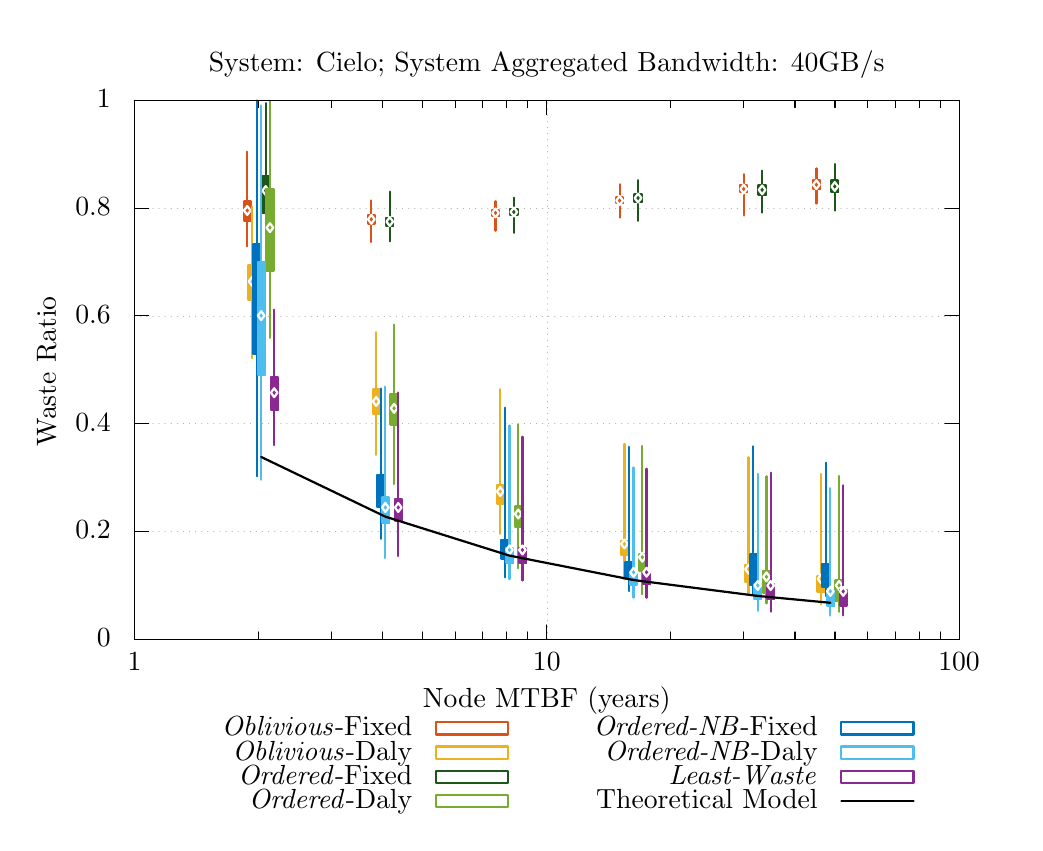
\begin{tikzpicture}[gnuplot]
%% generated with GNUPLOT 5.0p6 (Lua 5.3; terminal rev. 99, script rev. 100)
%% Thu Oct 19 16:09:22 2017
\path (0.000,0.000) rectangle (12.500,8.750);
\gpcolor{color=gp lt color axes}
\gpsetlinetype{gp lt axes}
\gpsetdashtype{gp dt axes}
\gpsetlinewidth{0.50}
\draw[gp path] (1.320,0.985)--(11.793,0.985);
\gpcolor{color=gp lt color border}
\gpsetlinetype{gp lt border}
\gpsetdashtype{gp dt solid}
\gpsetlinewidth{1.00}
\draw[gp path] (1.320,0.985)--(1.500,0.985);
\draw[gp path] (11.793,0.985)--(11.613,0.985);
\node[gp node right] at (1.136,0.985) {$0$};
\gpcolor{color=gp lt color axes}
\gpsetlinetype{gp lt axes}
\gpsetdashtype{gp dt axes}
\gpsetlinewidth{0.50}
\draw[gp path] (1.320,2.353)--(11.793,2.353);
\gpcolor{color=gp lt color border}
\gpsetlinetype{gp lt border}
\gpsetdashtype{gp dt solid}
\gpsetlinewidth{1.00}
\draw[gp path] (1.320,2.353)--(1.500,2.353);
\draw[gp path] (11.793,2.353)--(11.613,2.353);
\node[gp node right] at (1.136,2.353) {$0.2$};
\gpcolor{color=gp lt color axes}
\gpsetlinetype{gp lt axes}
\gpsetdashtype{gp dt axes}
\gpsetlinewidth{0.50}
\draw[gp path] (1.320,3.721)--(11.793,3.721);
\gpcolor{color=gp lt color border}
\gpsetlinetype{gp lt border}
\gpsetdashtype{gp dt solid}
\gpsetlinewidth{1.00}
\draw[gp path] (1.320,3.721)--(1.500,3.721);
\draw[gp path] (11.793,3.721)--(11.613,3.721);
\node[gp node right] at (1.136,3.721) {$0.4$};
\gpcolor{color=gp lt color axes}
\gpsetlinetype{gp lt axes}
\gpsetdashtype{gp dt axes}
\gpsetlinewidth{0.50}
\draw[gp path] (1.320,5.089)--(11.793,5.089);
\gpcolor{color=gp lt color border}
\gpsetlinetype{gp lt border}
\gpsetdashtype{gp dt solid}
\gpsetlinewidth{1.00}
\draw[gp path] (1.320,5.089)--(1.500,5.089);
\draw[gp path] (11.793,5.089)--(11.613,5.089);
\node[gp node right] at (1.136,5.089) {$0.6$};
\gpcolor{color=gp lt color axes}
\gpsetlinetype{gp lt axes}
\gpsetdashtype{gp dt axes}
\gpsetlinewidth{0.50}
\draw[gp path] (1.320,6.457)--(11.793,6.457);
\gpcolor{color=gp lt color border}
\gpsetlinetype{gp lt border}
\gpsetdashtype{gp dt solid}
\gpsetlinewidth{1.00}
\draw[gp path] (1.320,6.457)--(1.500,6.457);
\draw[gp path] (11.793,6.457)--(11.613,6.457);
\node[gp node right] at (1.136,6.457) {$0.8$};
\gpcolor{color=gp lt color axes}
\gpsetlinetype{gp lt axes}
\gpsetdashtype{gp dt axes}
\gpsetlinewidth{0.50}
\draw[gp path] (1.320,7.825)--(11.793,7.825);
\gpcolor{color=gp lt color border}
\gpsetlinetype{gp lt border}
\gpsetdashtype{gp dt solid}
\gpsetlinewidth{1.00}
\draw[gp path] (1.320,7.825)--(1.500,7.825);
\draw[gp path] (11.793,7.825)--(11.613,7.825);
\node[gp node right] at (1.136,7.825) {$1$};
\gpcolor{color=gp lt color axes}
\gpsetlinetype{gp lt axes}
\gpsetdashtype{gp dt axes}
\gpsetlinewidth{0.50}
\draw[gp path] (1.320,0.985)--(1.320,7.825);
\gpcolor{color=gp lt color border}
\gpsetlinetype{gp lt border}
\gpsetdashtype{gp dt solid}
\gpsetlinewidth{1.00}
\draw[gp path] (1.320,0.985)--(1.320,1.165);
\draw[gp path] (1.320,7.825)--(1.320,7.645);
\node[gp node center] at (1.320,0.677) {$1$};
\draw[gp path] (2.896,0.985)--(2.896,1.075);
\draw[gp path] (2.896,7.825)--(2.896,7.735);
\draw[gp path] (3.818,0.985)--(3.818,1.075);
\draw[gp path] (3.818,7.825)--(3.818,7.735);
\draw[gp path] (4.473,0.985)--(4.473,1.075);
\draw[gp path] (4.473,7.825)--(4.473,7.735);
\draw[gp path] (4.980,0.985)--(4.980,1.075);
\draw[gp path] (4.980,7.825)--(4.980,7.735);
\draw[gp path] (5.395,0.985)--(5.395,1.075);
\draw[gp path] (5.395,7.825)--(5.395,7.735);
\draw[gp path] (5.745,0.985)--(5.745,1.075);
\draw[gp path] (5.745,7.825)--(5.745,7.735);
\draw[gp path] (6.049,0.985)--(6.049,1.075);
\draw[gp path] (6.049,7.825)--(6.049,7.735);
\draw[gp path] (6.317,0.985)--(6.317,1.075);
\draw[gp path] (6.317,7.825)--(6.317,7.735);
\gpcolor{color=gp lt color axes}
\gpsetlinetype{gp lt axes}
\gpsetdashtype{gp dt axes}
\gpsetlinewidth{0.50}
\draw[gp path] (6.557,0.985)--(6.557,7.825);
\gpcolor{color=gp lt color border}
\gpsetlinetype{gp lt border}
\gpsetdashtype{gp dt solid}
\gpsetlinewidth{1.00}
\draw[gp path] (6.557,0.985)--(6.557,1.165);
\draw[gp path] (6.557,7.825)--(6.557,7.645);
\node[gp node center] at (6.557,0.677) {$10$};
\draw[gp path] (8.133,0.985)--(8.133,1.075);
\draw[gp path] (8.133,7.825)--(8.133,7.735);
\draw[gp path] (9.055,0.985)--(9.055,1.075);
\draw[gp path] (9.055,7.825)--(9.055,7.735);
\draw[gp path] (9.709,0.985)--(9.709,1.075);
\draw[gp path] (9.709,7.825)--(9.709,7.735);
\draw[gp path] (10.217,0.985)--(10.217,1.075);
\draw[gp path] (10.217,7.825)--(10.217,7.735);
\draw[gp path] (10.631,0.985)--(10.631,1.075);
\draw[gp path] (10.631,7.825)--(10.631,7.735);
\draw[gp path] (10.982,0.985)--(10.982,1.075);
\draw[gp path] (10.982,7.825)--(10.982,7.735);
\draw[gp path] (11.286,0.985)--(11.286,1.075);
\draw[gp path] (11.286,7.825)--(11.286,7.735);
\draw[gp path] (11.553,0.985)--(11.553,1.075);
\draw[gp path] (11.553,7.825)--(11.553,7.735);
\gpcolor{color=gp lt color axes}
\gpsetlinetype{gp lt axes}
\gpsetdashtype{gp dt axes}
\gpsetlinewidth{0.50}
\draw[gp path] (11.793,0.985)--(11.793,7.825);
\gpcolor{color=gp lt color border}
\gpsetlinetype{gp lt border}
\gpsetdashtype{gp dt solid}
\gpsetlinewidth{1.00}
\draw[gp path] (11.793,0.985)--(11.793,1.165);
\draw[gp path] (11.793,7.825)--(11.793,7.645);
\node[gp node center] at (11.793,0.677) {$100$};
\draw[gp path] (1.320,7.825)--(1.320,0.985)--(11.793,0.985)--(11.793,7.825)--cycle;
\node[gp node center,rotate=-270] at (0.246,4.405) {Waste Ratio};
\node[gp node center] at (6.556,0.215) {Node MTBF (years)};
\node[gp node center] at (6.556,8.287) {System: Cielo; System Aggregated Bandwidth: 40GB/s};
\node[gp node right] at (4.966,-0.149) {\propfixed};
\gpcolor{rgb color={0.851,0.325,0.098}}
\gpsetlinewidth{2.00}
\draw[gp path] (5.150,-0.226)--(6.066,-0.226)--(6.066,-0.072)--(5.150,-0.072)--cycle;
\gpfill{rgb color={0.851,0.325,0.098}} (2.708,6.295)--(2.798,6.295)--(2.798,6.541)--(2.708,6.541)--cycle;
\draw[gp path] (2.753,5.972)--(2.753,6.295);
\draw[gp path] (2.753,6.541)--(2.753,7.174);
\draw[gp path] (2.708,6.541)--(2.798,6.541)--(2.798,6.295)--(2.708,6.295)--cycle;
\gpfill{rgb color={0.851,0.325,0.098}} (4.284,6.263)--(4.374,6.263)--(4.374,6.370)--(4.284,6.370)--cycle;
\draw[gp path] (4.329,6.027)--(4.329,6.263);
\draw[gp path] (4.329,6.370)--(4.329,6.556);
\draw[gp path] (4.284,6.370)--(4.374,6.370)--(4.374,6.263)--(4.284,6.263)--cycle;
\gpfill{rgb color={0.851,0.325,0.098}} (5.861,6.363)--(5.951,6.363)--(5.951,6.437)--(5.861,6.437)--cycle;
\draw[gp path] (5.906,6.172)--(5.906,6.363);
\draw[gp path] (5.906,6.437)--(5.906,6.546);
\draw[gp path] (5.861,6.437)--(5.951,6.437)--(5.951,6.363)--(5.861,6.363)--cycle;
\gpfill{rgb color={0.851,0.325,0.098}} (7.437,6.519)--(7.527,6.519)--(7.527,6.593)--(7.437,6.593)--cycle;
\draw[gp path] (7.482,6.339)--(7.482,6.519);
\draw[gp path] (7.482,6.593)--(7.482,6.761);
\draw[gp path] (7.437,6.593)--(7.527,6.593)--(7.527,6.519)--(7.437,6.519)--cycle;
\gpfill{rgb color={0.851,0.325,0.098}} (9.013,6.658)--(9.103,6.658)--(9.103,6.754)--(9.013,6.754)--cycle;
\draw[gp path] (9.058,6.365)--(9.058,6.658);
\draw[gp path] (9.058,6.754)--(9.058,6.889);
\draw[gp path] (9.013,6.754)--(9.103,6.754)--(9.103,6.658)--(9.013,6.658)--cycle;
\gpfill{rgb color={0.851,0.325,0.098}} (9.936,6.701)--(10.026,6.701)--(10.026,6.813)--(9.936,6.813)--cycle;
\draw[gp path] (9.981,6.516)--(9.981,6.701);
\draw[gp path] (9.981,6.813)--(9.981,6.963);
\draw[gp path] (9.936,6.813)--(10.026,6.813)--(10.026,6.701)--(9.936,6.701)--cycle;
\gpcolor{rgb color={1.000,1.000,1.000}}
\gpsetpointsize{4.00}
\gppoint{gp mark 12}{(2.753,6.428)}
\gppoint{gp mark 12}{(4.329,6.316)}
\gppoint{gp mark 12}{(5.906,6.397)}
\gppoint{gp mark 12}{(7.482,6.554)}
\gppoint{gp mark 12}{(9.058,6.701)}
\gppoint{gp mark 12}{(9.981,6.756)}
\gpcolor{color=gp lt color border}
\node[gp node right] at (4.966,-0.457) {\propdaly};
\gpcolor{rgb color={0.929,0.694,0.125}}
\draw[gp path] (5.150,-0.534)--(6.066,-0.534)--(6.066,-0.380)--(5.150,-0.380)--cycle;
\gpfill{rgb color={0.929,0.694,0.125}} (2.769,5.296)--(2.859,5.296)--(2.859,5.740)--(2.769,5.740)--cycle;
\draw[gp path] (2.814,4.554)--(2.814,5.296);
\draw[gp path] (2.814,5.740)--(2.814,6.476);
\draw[gp path] (2.769,5.740)--(2.859,5.740)--(2.859,5.296)--(2.769,5.296)--cycle;
\gpfill{rgb color={0.929,0.694,0.125}} (4.345,3.847)--(4.435,3.847)--(4.435,4.156)--(4.345,4.156)--cycle;
\draw[gp path] (4.390,3.324)--(4.390,3.847);
\draw[gp path] (4.390,4.156)--(4.390,4.883);
\draw[gp path] (4.345,4.156)--(4.435,4.156)--(4.435,3.847)--(4.345,3.847)--cycle;
\gpfill{rgb color={0.929,0.694,0.125}} (5.921,2.708)--(6.011,2.708)--(6.011,2.943)--(5.921,2.943)--cycle;
\draw[gp path] (5.966,2.323)--(5.966,2.708);
\draw[gp path] (5.966,2.943)--(5.966,4.159);
\draw[gp path] (5.921,2.943)--(6.011,2.943)--(6.011,2.708)--(5.921,2.708)--cycle;
\gpfill{rgb color={0.929,0.694,0.125}} (7.498,2.053)--(7.588,2.053)--(7.588,2.233)--(7.498,2.233)--cycle;
\draw[gp path] (7.543,1.743)--(7.543,2.053);
\draw[gp path] (7.543,2.233)--(7.543,3.462);
\draw[gp path] (7.498,2.233)--(7.588,2.233)--(7.588,2.053)--(7.498,2.053)--cycle;
\gpfill{rgb color={0.929,0.694,0.125}} (9.074,1.712)--(9.164,1.712)--(9.164,1.922)--(9.074,1.922)--cycle;
\draw[gp path] (9.119,1.545)--(9.119,1.712);
\draw[gp path] (9.119,1.922)--(9.119,3.295);
\draw[gp path] (9.074,1.922)--(9.164,1.922)--(9.164,1.712)--(9.074,1.712)--cycle;
\gpfill{rgb color={0.929,0.694,0.125}} (9.996,1.579)--(10.086,1.579)--(10.086,1.785)--(9.996,1.785)--cycle;
\draw[gp path] (10.041,1.426)--(10.041,1.579);
\draw[gp path] (10.041,1.785)--(10.041,3.082);
\draw[gp path] (9.996,1.785)--(10.086,1.785)--(10.086,1.579)--(9.996,1.579)--cycle;
\gpcolor{rgb color={1.000,1.000,1.000}}
\gppoint{gp mark 12}{(2.814,5.528)}
\gppoint{gp mark 12}{(4.390,4.003)}
\gppoint{gp mark 12}{(5.966,2.859)}
\gppoint{gp mark 12}{(7.543,2.193)}
\gppoint{gp mark 12}{(9.119,1.873)}
\gppoint{gp mark 12}{(10.041,1.751)}
\gpcolor{color=gp lt color border}
\node[gp node right] at (4.966,-0.765) {\bfifofixed};
\gpcolor{rgb color={0.110,0.337,0.094}}
\draw[gp path] (5.150,-0.842)--(6.066,-0.842)--(6.066,-0.688)--(5.150,-0.688)--cycle;
\gpfill{rgb color={0.110,0.337,0.094}} (2.942,6.397)--(3.032,6.397)--(3.032,6.864)--(2.942,6.864)--cycle;
\draw[gp path] (2.987,6.053)--(2.987,6.397);
\draw[gp path] (2.987,6.864)--(2.987,7.790);
\draw[gp path] (2.942,6.864)--(3.032,6.864)--(3.032,6.397)--(2.942,6.397)--cycle;
\gpfill{rgb color={0.110,0.337,0.094}} (4.518,6.234)--(4.608,6.234)--(4.608,6.332)--(4.518,6.332)--cycle;
\draw[gp path] (4.563,6.037)--(4.563,6.234);
\draw[gp path] (4.563,6.332)--(4.563,6.668);
\draw[gp path] (4.518,6.332)--(4.608,6.332)--(4.608,6.234)--(4.518,6.234)--cycle;
\gpfill{rgb color={0.110,0.337,0.094}} (6.094,6.373)--(6.184,6.373)--(6.184,6.447)--(6.094,6.447)--cycle;
\draw[gp path] (6.139,6.145)--(6.139,6.373);
\draw[gp path] (6.139,6.447)--(6.139,6.590);
\draw[gp path] (6.094,6.447)--(6.184,6.447)--(6.184,6.373)--(6.094,6.373)--cycle;
\gpfill{rgb color={0.110,0.337,0.094}} (7.671,6.535)--(7.761,6.535)--(7.761,6.640)--(7.671,6.640)--cycle;
\draw[gp path] (7.716,6.297)--(7.716,6.535);
\draw[gp path] (7.716,6.640)--(7.716,6.812);
\draw[gp path] (7.671,6.640)--(7.761,6.640)--(7.761,6.535)--(7.671,6.535)--cycle;
\gpfill{rgb color={0.110,0.337,0.094}} (9.247,6.629)--(9.337,6.629)--(9.337,6.752)--(9.247,6.752)--cycle;
\draw[gp path] (9.292,6.402)--(9.292,6.629);
\draw[gp path] (9.292,6.752)--(9.292,6.935);
\draw[gp path] (9.247,6.752)--(9.337,6.752)--(9.337,6.629)--(9.247,6.629)--cycle;
\gpfill{rgb color={0.110,0.337,0.094}} (10.169,6.658)--(10.259,6.658)--(10.259,6.808)--(10.169,6.808)--cycle;
\draw[gp path] (10.214,6.428)--(10.214,6.658);
\draw[gp path] (10.214,6.808)--(10.214,7.018);
\draw[gp path] (10.169,6.808)--(10.259,6.808)--(10.259,6.658)--(10.169,6.658)--cycle;
\gpcolor{rgb color={1.000,1.000,1.000}}
\gppoint{gp mark 12}{(2.987,6.681)}
\gppoint{gp mark 12}{(4.563,6.287)}
\gppoint{gp mark 12}{(6.139,6.409)}
\gppoint{gp mark 12}{(7.716,6.586)}
\gppoint{gp mark 12}{(9.292,6.690)}
\gppoint{gp mark 12}{(10.214,6.733)}
\gpcolor{color=gp lt color border}
\node[gp node right] at (4.966,-1.073) {\bfifodaly};
\gpcolor{rgb color={0.467,0.675,0.188}}
\draw[gp path] (5.150,-1.150)--(6.066,-1.150)--(6.066,-0.996)--(5.150,-0.996)--cycle;
\gpfill{rgb color={0.467,0.675,0.188}} (2.996,5.660)--(3.086,5.660)--(3.086,6.697)--(2.996,6.697)--cycle;
\draw[gp path] (3.041,4.810)--(3.041,5.660);
\draw[gp path] (3.041,6.697)--(3.041,7.824);
\draw[gp path] (2.996,6.697)--(3.086,6.697)--(3.086,5.660)--(2.996,5.660)--cycle;
\gpfill{rgb color={0.467,0.675,0.188}} (4.573,3.711)--(4.663,3.711)--(4.663,4.102)--(4.573,4.102)--cycle;
\draw[gp path] (4.618,2.955)--(4.618,3.711);
\draw[gp path] (4.618,4.102)--(4.618,4.977);
\draw[gp path] (4.573,4.102)--(4.663,4.102)--(4.663,3.711)--(4.573,3.711)--cycle;
\gpfill{rgb color={0.467,0.675,0.188}} (6.149,2.408)--(6.239,2.408)--(6.239,2.668)--(6.149,2.668)--cycle;
\draw[gp path] (6.194,1.885)--(6.194,2.408);
\draw[gp path] (6.194,2.668)--(6.194,3.712);
\draw[gp path] (6.149,2.668)--(6.239,2.668)--(6.239,2.408)--(6.149,2.408)--cycle;
\gpfill{rgb color={0.467,0.675,0.188}} (7.725,1.856)--(7.815,1.856)--(7.815,2.059)--(7.725,2.059)--cycle;
\draw[gp path] (7.770,1.555)--(7.770,1.856);
\draw[gp path] (7.770,2.059)--(7.770,3.437);
\draw[gp path] (7.725,2.059)--(7.815,2.059)--(7.815,1.856)--(7.725,1.856)--cycle;
\gpfill{rgb color={0.467,0.675,0.188}} (9.302,1.575)--(9.392,1.575)--(9.392,1.849)--(9.302,1.849)--cycle;
\draw[gp path] (9.347,1.439)--(9.347,1.575);
\draw[gp path] (9.347,1.849)--(9.347,3.052);
\draw[gp path] (9.302,1.849)--(9.392,1.849)--(9.392,1.575)--(9.302,1.575)--cycle;
\gpfill{rgb color={0.467,0.675,0.188}} (10.224,1.465)--(10.314,1.465)--(10.314,1.729)--(10.224,1.729)--cycle;
\draw[gp path] (10.269,1.332)--(10.269,1.465);
\draw[gp path] (10.269,1.729)--(10.269,3.056);
\draw[gp path] (10.224,1.729)--(10.314,1.729)--(10.314,1.465)--(10.224,1.465)--cycle;
\gpcolor{rgb color={1.000,1.000,1.000}}
\gppoint{gp mark 12}{(3.041,6.210)}
\gppoint{gp mark 12}{(4.618,3.916)}
\gppoint{gp mark 12}{(6.194,2.574)}
\gppoint{gp mark 12}{(7.770,2.025)}
\gppoint{gp mark 12}{(9.347,1.776)}
\gppoint{gp mark 12}{(10.269,1.667)}
\gpcolor{color=gp lt color border}
\node[gp node right] at (10.114,-0.149) {\fifofixed};
\gpcolor{rgb color={0.000,0.447,0.741}}
\draw[gp path] (10.298,-0.226)--(11.214,-0.226)--(11.214,-0.072)--(10.298,-0.072)--cycle;
\gpfill{rgb color={0.000,0.447,0.741}} (2.828,4.608)--(2.918,4.608)--(2.918,5.997)--(2.828,5.997)--cycle;
\draw[gp path] (2.873,3.053)--(2.873,4.608);
\draw[gp path] (2.873,5.997)--(2.873,7.825);
\draw[gp path] (2.828,5.997)--(2.918,5.997)--(2.918,4.608)--(2.828,4.608)--cycle;
\gpfill{rgb color={0.000,0.447,0.741}} (4.404,2.667)--(4.494,2.667)--(4.494,3.073)--(4.404,3.073)--cycle;
\draw[gp path] (4.449,2.259)--(4.449,2.667);
\draw[gp path] (4.449,3.073)--(4.449,4.167);
\draw[gp path] (4.404,3.073)--(4.494,3.073)--(4.494,2.667)--(4.404,2.667)--cycle;
\gpfill{rgb color={0.000,0.447,0.741}} (5.980,2.009)--(6.070,2.009)--(6.070,2.241)--(5.980,2.241)--cycle;
\draw[gp path] (6.025,1.768)--(6.025,2.009);
\draw[gp path] (6.025,2.241)--(6.025,3.923);
\draw[gp path] (5.980,2.241)--(6.070,2.241)--(6.070,2.009)--(5.980,2.009)--cycle;
\gpfill{rgb color={0.000,0.447,0.741}} (7.557,1.770)--(7.647,1.770)--(7.647,1.961)--(7.557,1.961)--cycle;
\draw[gp path] (7.602,1.594)--(7.602,1.770);
\draw[gp path] (7.602,1.961)--(7.602,3.427);
\draw[gp path] (7.557,1.961)--(7.647,1.961)--(7.647,1.770)--(7.557,1.770)--cycle;
\gpfill{rgb color={0.000,0.447,0.741}} (9.133,1.676)--(9.223,1.676)--(9.223,2.060)--(9.133,2.060)--cycle;
\draw[gp path] (9.178,1.555)--(9.178,1.676);
\draw[gp path] (9.178,2.060)--(9.178,3.433);
\draw[gp path] (9.133,2.060)--(9.223,2.060)--(9.223,1.676)--(9.133,1.676)--cycle;
\gpfill{rgb color={0.000,0.447,0.741}} (10.055,1.652)--(10.145,1.652)--(10.145,1.939)--(10.055,1.939)--cycle;
\draw[gp path] (10.100,1.532)--(10.100,1.652);
\draw[gp path] (10.100,1.939)--(10.100,3.226);
\draw[gp path] (10.055,1.939)--(10.145,1.939)--(10.145,1.652)--(10.055,1.652)--cycle;
\gpcolor{color=gp lt color border}
\node[gp node right] at (10.114,-0.457) {\fifodaly};
\gpcolor{rgb color={0.302,0.745,0.933}}
\draw[gp path] (10.298,-0.534)--(11.214,-0.534)--(11.214,-0.380)--(10.298,-0.380)--cycle;
\gpfill{rgb color={0.302,0.745,0.933}} (2.885,4.342)--(2.975,4.342)--(2.975,5.777)--(2.885,5.777)--cycle;
\draw[gp path] (2.930,3.009)--(2.930,4.342);
\draw[gp path] (2.930,5.777)--(2.930,7.761);
\draw[gp path] (2.885,5.777)--(2.975,5.777)--(2.975,4.342)--(2.885,4.342)--cycle;
\gpfill{rgb color={0.302,0.745,0.933}} (4.462,2.459)--(4.552,2.459)--(4.552,2.782)--(4.462,2.782)--cycle;
\draw[gp path] (4.507,2.014)--(4.507,2.459);
\draw[gp path] (4.507,2.782)--(4.507,4.192);
\draw[gp path] (4.462,2.782)--(4.552,2.782)--(4.552,2.459)--(4.462,2.459)--cycle;
\gpfill{rgb color={0.302,0.745,0.933}} (6.038,1.951)--(6.128,1.951)--(6.128,2.143)--(6.038,2.143)--cycle;
\draw[gp path] (6.083,1.748)--(6.083,1.951);
\draw[gp path] (6.083,2.143)--(6.083,3.697);
\draw[gp path] (6.038,2.143)--(6.128,2.143)--(6.128,1.951)--(6.038,1.951)--cycle;
\gpfill{rgb color={0.302,0.745,0.933}} (7.614,1.679)--(7.704,1.679)--(7.704,1.830)--(7.614,1.830)--cycle;
\draw[gp path] (7.659,1.512)--(7.659,1.679);
\draw[gp path] (7.659,1.830)--(7.659,3.164);
\draw[gp path] (7.614,1.830)--(7.704,1.830)--(7.704,1.679)--(7.614,1.679)--cycle;
\gpfill{rgb color={0.302,0.745,0.933}} (9.191,1.494)--(9.281,1.494)--(9.281,1.679)--(9.191,1.679)--cycle;
\draw[gp path] (9.236,1.345)--(9.236,1.494);
\draw[gp path] (9.236,1.679)--(9.236,3.084);
\draw[gp path] (9.191,1.679)--(9.281,1.679)--(9.281,1.494)--(9.191,1.494)--cycle;
\gpfill{rgb color={0.302,0.745,0.933}} (10.113,1.408)--(10.203,1.408)--(10.203,1.604)--(10.113,1.604)--cycle;
\draw[gp path] (10.158,1.285)--(10.158,1.408);
\draw[gp path] (10.158,1.604)--(10.158,2.901);
\draw[gp path] (10.113,1.604)--(10.203,1.604)--(10.203,1.408)--(10.113,1.408)--cycle;
\gpcolor{rgb color={1.000,1.000,1.000}}
\gppoint{gp mark 12}{(2.930,5.093)}
\gppoint{gp mark 12}{(4.507,2.657)}
\gppoint{gp mark 12}{(6.083,2.118)}
\gppoint{gp mark 12}{(7.659,1.833)}
\gppoint{gp mark 12}{(9.236,1.666)}
\gppoint{gp mark 12}{(10.158,1.591)}
\gpcolor{color=gp lt color border}
\node[gp node right] at (10.114,-0.765) {\cooperative};
\gpcolor{rgb color={0.545,0.161,0.573}}
\draw[gp path] (10.298,-0.842)--(11.214,-0.842)--(11.214,-0.688)--(10.298,-0.688)--cycle;
\gpfill{rgb color={0.545,0.161,0.573}} (3.050,3.897)--(3.140,3.897)--(3.140,4.315)--(3.050,4.315)--cycle;
\draw[gp path] (3.095,3.448)--(3.095,3.897);
\draw[gp path] (3.095,4.315)--(3.095,5.168);
\draw[gp path] (3.050,4.315)--(3.140,4.315)--(3.140,3.897)--(3.050,3.897)--cycle;
\gpfill{rgb color={0.545,0.161,0.573}} (4.626,2.483)--(4.716,2.483)--(4.716,2.762)--(4.626,2.762)--cycle;
\draw[gp path] (4.671,2.040)--(4.671,2.483);
\draw[gp path] (4.671,2.762)--(4.671,4.116);
\draw[gp path] (4.626,2.762)--(4.716,2.762)--(4.716,2.483)--(4.626,2.483)--cycle;
\gpfill{rgb color={0.545,0.161,0.573}} (6.203,1.950)--(6.293,1.950)--(6.293,2.135)--(6.203,2.135)--cycle;
\draw[gp path] (6.248,1.730)--(6.248,1.950);
\draw[gp path] (6.248,2.135)--(6.248,3.554);
\draw[gp path] (6.203,2.135)--(6.293,2.135)--(6.293,1.950)--(6.203,1.950)--cycle;
\gpfill{rgb color={0.545,0.161,0.573}} (7.779,1.682)--(7.869,1.682)--(7.869,1.826)--(7.779,1.826)--cycle;
\draw[gp path] (7.824,1.510)--(7.824,1.682);
\draw[gp path] (7.824,1.826)--(7.824,3.147);
\draw[gp path] (7.779,1.826)--(7.869,1.826)--(7.869,1.682)--(7.779,1.682)--cycle;
\gpfill{rgb color={0.545,0.161,0.573}} (9.355,1.492)--(9.445,1.492)--(9.445,1.685)--(9.355,1.685)--cycle;
\draw[gp path] (9.400,1.333)--(9.400,1.492);
\draw[gp path] (9.400,1.685)--(9.400,3.099);
\draw[gp path] (9.355,1.685)--(9.445,1.685)--(9.445,1.492)--(9.355,1.492)--cycle;
\gpfill{rgb color={0.545,0.161,0.573}} (10.277,1.412)--(10.367,1.412)--(10.367,1.606)--(10.277,1.606)--cycle;
\draw[gp path] (10.322,1.286)--(10.322,1.412);
\draw[gp path] (10.322,1.606)--(10.322,2.938);
\draw[gp path] (10.277,1.606)--(10.367,1.606)--(10.367,1.412)--(10.277,1.412)--cycle;
\gpcolor{rgb color={1.000,1.000,1.000}}
\gppoint{gp mark 12}{(3.095,4.114)}
\gppoint{gp mark 12}{(4.671,2.656)}
\gppoint{gp mark 12}{(6.248,2.117)}
\gppoint{gp mark 12}{(7.824,1.834)}
\gppoint{gp mark 12}{(9.400,1.665)}
\gppoint{gp mark 12}{(10.322,1.590)}
\gpcolor{color=gp lt color border}
\node[gp node right] at (10.114,-1.073) {Theoretical Model};
\gpcolor{rgb color={0.000,0.000,0.000}}
\draw[gp path] (10.298,-1.073)--(11.214,-1.073);
\draw[gp path] (2.930,3.298)--(4.507,2.540)--(6.083,2.045)--(7.659,1.735)--(9.236,1.533)%
  --(10.158,1.446);
\gpcolor{color=gp lt color border}
\gpsetlinewidth{1.00}
\draw[gp path] (1.320,7.825)--(1.320,0.985)--(11.793,0.985)--(11.793,7.825)--cycle;
%% coordinates of the plot area
\gpdefrectangularnode{gp plot 1}{\pgfpoint{1.320cm}{0.985cm}}{\pgfpoint{11.793cm}{7.825cm}}
\end{tikzpicture}
%% gnuplot variables
}
    
    $\bandavail=40 \text{GBs}$
  \end{center}
 
       \end{frame}

    
      \begin{frame}
  \frametitle{Prospective system (1/2)}
 
 \begin{itemize}
\item Aurora-like\\
7PB of main memory and 50,000 compute nodes 
\item Scale APEX workflow\\
accordingly to Aurora/Celio memory size increase 

\end{itemize}

 
       \end{frame}
       
      \begin{frame}
       \frametitle{Prospective system (2/2)}


 
  \begin{center}
    \resizebox{0.95\linewidth}{!}{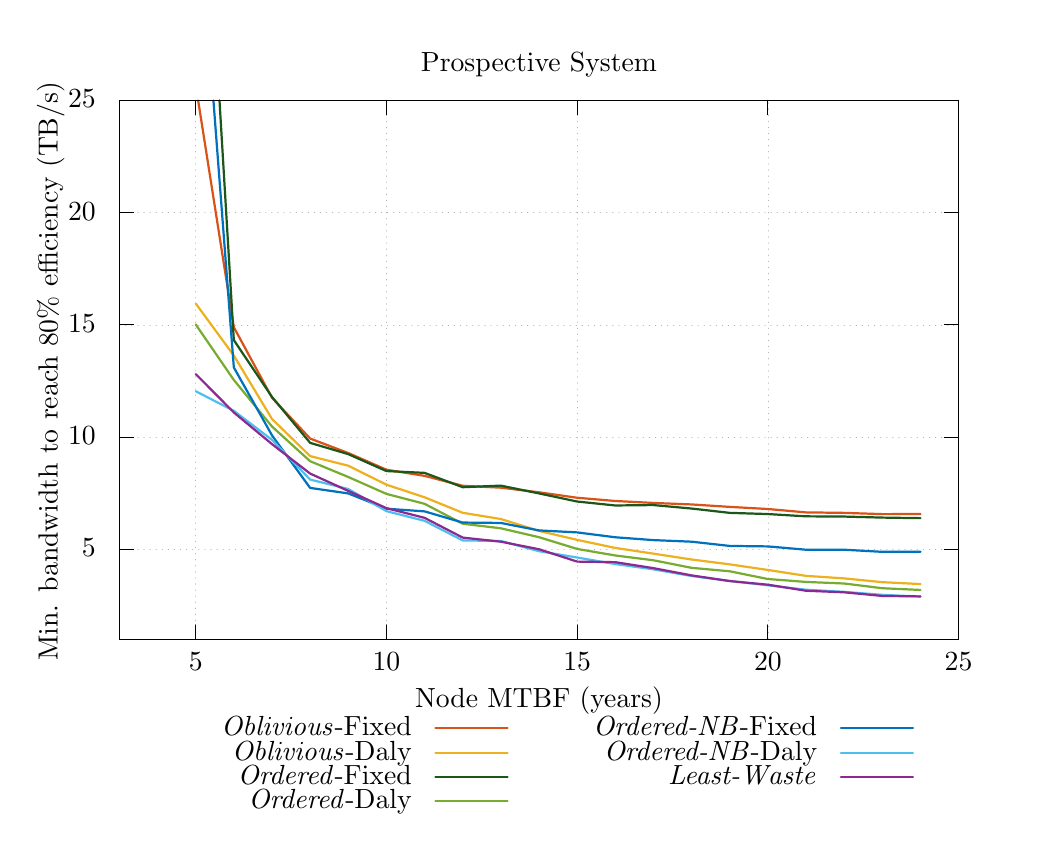
\begin{tikzpicture}[gnuplot]
%% generated with GNUPLOT 5.2p0 (Lua 5.3; terminal rev. 99, script rev. 102)
%% Thu Oct 19 14:13:35 2017
\path (0.000,0.000) rectangle (12.500,8.750);
\gpcolor{color=gp lt color axes}
\gpsetlinetype{gp lt axes}
\gpsetdashtype{gp dt axes}
\gpsetlinewidth{0.50}
\draw[gp path] (1.136,2.125)--(11.793,2.125);
\gpcolor{color=gp lt color border}
\gpsetlinetype{gp lt border}
\gpsetdashtype{gp dt solid}
\gpsetlinewidth{1.00}
\draw[gp path] (1.136,2.125)--(1.316,2.125);
\draw[gp path] (11.793,2.125)--(11.613,2.125);
\node[gp node right] at (0.952,2.125) {$5$};
\gpcolor{color=gp lt color axes}
\gpsetlinetype{gp lt axes}
\gpsetdashtype{gp dt axes}
\gpsetlinewidth{0.50}
\draw[gp path] (1.136,3.550)--(11.793,3.550);
\gpcolor{color=gp lt color border}
\gpsetlinetype{gp lt border}
\gpsetdashtype{gp dt solid}
\gpsetlinewidth{1.00}
\draw[gp path] (1.136,3.550)--(1.316,3.550);
\draw[gp path] (11.793,3.550)--(11.613,3.550);
\node[gp node right] at (0.952,3.550) {$10$};
\gpcolor{color=gp lt color axes}
\gpsetlinetype{gp lt axes}
\gpsetdashtype{gp dt axes}
\gpsetlinewidth{0.50}
\draw[gp path] (1.136,4.975)--(11.793,4.975);
\gpcolor{color=gp lt color border}
\gpsetlinetype{gp lt border}
\gpsetdashtype{gp dt solid}
\gpsetlinewidth{1.00}
\draw[gp path] (1.136,4.975)--(1.316,4.975);
\draw[gp path] (11.793,4.975)--(11.613,4.975);
\node[gp node right] at (0.952,4.975) {$15$};
\gpcolor{color=gp lt color axes}
\gpsetlinetype{gp lt axes}
\gpsetdashtype{gp dt axes}
\gpsetlinewidth{0.50}
\draw[gp path] (1.136,6.400)--(11.793,6.400);
\gpcolor{color=gp lt color border}
\gpsetlinetype{gp lt border}
\gpsetdashtype{gp dt solid}
\gpsetlinewidth{1.00}
\draw[gp path] (1.136,6.400)--(1.316,6.400);
\draw[gp path] (11.793,6.400)--(11.613,6.400);
\node[gp node right] at (0.952,6.400) {$20$};
\gpcolor{color=gp lt color axes}
\gpsetlinetype{gp lt axes}
\gpsetdashtype{gp dt axes}
\gpsetlinewidth{0.50}
\draw[gp path] (1.136,7.825)--(11.793,7.825);
\gpcolor{color=gp lt color border}
\gpsetlinetype{gp lt border}
\gpsetdashtype{gp dt solid}
\gpsetlinewidth{1.00}
\draw[gp path] (1.136,7.825)--(1.316,7.825);
\draw[gp path] (11.793,7.825)--(11.613,7.825);
\node[gp node right] at (0.952,7.825) {$25$};
\gpcolor{color=gp lt color axes}
\gpsetlinetype{gp lt axes}
\gpsetdashtype{gp dt axes}
\gpsetlinewidth{0.50}
\draw[gp path] (2.105,0.985)--(2.105,7.825);
\gpcolor{color=gp lt color border}
\gpsetlinetype{gp lt border}
\gpsetdashtype{gp dt solid}
\gpsetlinewidth{1.00}
\draw[gp path] (2.105,0.985)--(2.105,1.165);
\draw[gp path] (2.105,7.825)--(2.105,7.645);
\node[gp node center] at (2.105,0.677) {$5$};
\gpcolor{color=gp lt color axes}
\gpsetlinetype{gp lt axes}
\gpsetdashtype{gp dt axes}
\gpsetlinewidth{0.50}
\draw[gp path] (4.527,0.985)--(4.527,7.825);
\gpcolor{color=gp lt color border}
\gpsetlinetype{gp lt border}
\gpsetdashtype{gp dt solid}
\gpsetlinewidth{1.00}
\draw[gp path] (4.527,0.985)--(4.527,1.165);
\draw[gp path] (4.527,7.825)--(4.527,7.645);
\node[gp node center] at (4.527,0.677) {$10$};
\gpcolor{color=gp lt color axes}
\gpsetlinetype{gp lt axes}
\gpsetdashtype{gp dt axes}
\gpsetlinewidth{0.50}
\draw[gp path] (6.949,0.985)--(6.949,7.825);
\gpcolor{color=gp lt color border}
\gpsetlinetype{gp lt border}
\gpsetdashtype{gp dt solid}
\gpsetlinewidth{1.00}
\draw[gp path] (6.949,0.985)--(6.949,1.165);
\draw[gp path] (6.949,7.825)--(6.949,7.645);
\node[gp node center] at (6.949,0.677) {$15$};
\gpcolor{color=gp lt color axes}
\gpsetlinetype{gp lt axes}
\gpsetdashtype{gp dt axes}
\gpsetlinewidth{0.50}
\draw[gp path] (9.371,0.985)--(9.371,7.825);
\gpcolor{color=gp lt color border}
\gpsetlinetype{gp lt border}
\gpsetdashtype{gp dt solid}
\gpsetlinewidth{1.00}
\draw[gp path] (9.371,0.985)--(9.371,1.165);
\draw[gp path] (9.371,7.825)--(9.371,7.645);
\node[gp node center] at (9.371,0.677) {$20$};
\gpcolor{color=gp lt color axes}
\gpsetlinetype{gp lt axes}
\gpsetdashtype{gp dt axes}
\gpsetlinewidth{0.50}
\draw[gp path] (11.793,0.985)--(11.793,7.825);
\gpcolor{color=gp lt color border}
\gpsetlinetype{gp lt border}
\gpsetdashtype{gp dt solid}
\gpsetlinewidth{1.00}
\draw[gp path] (11.793,0.985)--(11.793,1.165);
\draw[gp path] (11.793,7.825)--(11.793,7.645);
\node[gp node center] at (11.793,0.677) {$25$};
\draw[gp path] (1.136,7.825)--(1.136,0.985)--(11.793,0.985)--(11.793,7.825)--cycle;
\node[gp node center,rotate=-270] at (0.276,4.405) {Min. bandwidth to reach 80\% efficiency (TB/s)};
\node[gp node center] at (6.464,0.215) {Node MTBF (years)};
\node[gp node center] at (6.464,8.287) {Prospective System};
\node[gp node right] at (4.966,-0.149) {\propfixed};
\gpcolor{rgb color={0.851,0.325,0.098}}
\gpsetlinewidth{2.00}
\draw[gp path] (5.150,-0.149)--(6.066,-0.149);
\draw[gp path] (2.136,7.825)--(2.589,4.946)--(3.074,4.050)--(3.558,3.532)--(4.042,3.348)%
  --(4.527,3.136)--(5.011,3.058)--(5.496,2.932)--(5.980,2.908)--(6.465,2.849)--(6.949,2.780)%
  --(7.433,2.739)--(7.918,2.714)--(8.402,2.695)--(8.887,2.664)--(9.371,2.637)--(9.855,2.594)%
  --(10.340,2.588)--(10.824,2.572)--(11.309,2.573);
\gpcolor{color=gp lt color border}
\node[gp node right] at (4.966,-0.457) {\propdaly};
\gpcolor{rgb color={0.929,0.694,0.125}}
\draw[gp path] (5.150,-0.457)--(6.066,-0.457);
\draw[gp path] (2.105,5.247)--(2.589,4.586)--(3.074,3.780)--(3.558,3.309)--(4.042,3.187)%
  --(4.527,2.946)--(5.011,2.786)--(5.496,2.589)--(5.980,2.510)--(6.465,2.359)--(6.949,2.245)%
  --(7.433,2.143)--(7.918,2.070)--(8.402,1.996)--(8.887,1.934)--(9.371,1.863)--(9.855,1.788)%
  --(10.340,1.756)--(10.824,1.708)--(11.309,1.684);
\gpcolor{color=gp lt color border}
\node[gp node right] at (4.966,-0.765) {\bfifofixed};
\gpcolor{rgb color={0.110,0.337,0.094}}
\draw[gp path] (5.150,-0.765)--(6.066,-0.765);
\draw[gp path] (2.407,7.825)--(2.589,4.782)--(3.074,4.060)--(3.558,3.477)--(4.042,3.334)%
  --(4.527,3.119)--(5.011,3.096)--(5.496,2.914)--(5.980,2.934)--(6.465,2.835)--(6.949,2.732)%
  --(7.433,2.682)--(7.918,2.687)--(8.402,2.643)--(8.887,2.588)--(9.371,2.573)--(9.855,2.544)%
  --(10.340,2.541)--(10.824,2.528)--(11.309,2.521);
\gpcolor{color=gp lt color border}
\node[gp node right] at (4.966,-1.073) {\bfifodaly};
\gpcolor{rgb color={0.467,0.675,0.188}}
\draw[gp path] (5.150,-1.073)--(6.066,-1.073);
\draw[gp path] (2.105,4.981)--(2.589,4.276)--(3.074,3.684)--(3.558,3.244)--(4.042,3.044)%
  --(4.527,2.829)--(5.011,2.703)--(5.496,2.450)--(5.980,2.392)--(6.465,2.279)--(6.949,2.130)%
  --(7.433,2.047)--(7.918,1.986)--(8.402,1.890)--(8.887,1.846)--(9.371,1.748)--(9.855,1.711)%
  --(10.340,1.691)--(10.824,1.631)--(11.309,1.609);
\gpcolor{color=gp lt color border}
\node[gp node right] at (10.114,-0.149) {\fifofixed};
\gpcolor{rgb color={0.000,0.447,0.741}}
\draw[gp path] (10.298,-0.149)--(11.214,-0.149);
\draw[gp path] (2.330,7.825)--(2.589,4.435)--(3.074,3.572)--(3.558,2.905)--(4.042,2.835)%
  --(4.527,2.641)--(5.011,2.607)--(5.496,2.465)--(5.980,2.460)--(6.465,2.365)--(6.949,2.340)%
  --(7.433,2.278)--(7.918,2.242)--(8.402,2.222)--(8.887,2.168)--(9.371,2.162)--(9.855,2.120)%
  --(10.340,2.120)--(10.824,2.093)--(11.309,2.094);
\gpcolor{color=gp lt color border}
\node[gp node right] at (10.114,-0.457) {\fifodaly};
\gpcolor{rgb color={0.302,0.745,0.933}}
\draw[gp path] (10.298,-0.457)--(11.214,-0.457);
\draw[gp path] (2.105,4.133)--(2.589,3.884)--(3.074,3.515)--(3.558,3.011)--(4.042,2.891)%
  --(4.527,2.610)--(5.011,2.487)--(5.496,2.238)--(5.980,2.231)--(6.465,2.101)--(6.949,2.021)%
  --(7.433,1.938)--(7.918,1.871)--(8.402,1.786)--(8.887,1.723)--(9.371,1.668)--(9.855,1.612)%
  --(10.340,1.585)--(10.824,1.547)--(11.309,1.525);
\gpcolor{color=gp lt color border}
\node[gp node right] at (10.114,-0.765) {\cooperative};
\gpcolor{rgb color={0.545,0.161,0.573}}
\draw[gp path] (10.298,-0.765)--(11.214,-0.765);
\draw[gp path] (2.105,4.351)--(2.589,3.863)--(3.074,3.461)--(3.558,3.087)--(4.042,2.867)%
  --(4.527,2.648)--(5.011,2.525)--(5.496,2.274)--(5.980,2.222)--(6.465,2.126)--(6.949,1.969)%
  --(7.433,1.962)--(7.918,1.886)--(8.402,1.794)--(8.887,1.722)--(9.371,1.676)--(9.855,1.599)%
  --(10.340,1.579)--(10.824,1.533)--(11.309,1.527);
\gpcolor{color=gp lt color border}
\gpsetlinewidth{1.00}
\draw[gp path] (1.136,7.825)--(1.136,0.985)--(11.793,0.985)--(11.793,7.825)--cycle;
%% coordinates of the plot area
\gpdefrectangularnode{gp plot 1}{\pgfpoint{1.136cm}{0.985cm}}{\pgfpoint{11.793cm}{7.825cm}}
\end{tikzpicture}
%% gnuplot variables
}
  \end{center}
 
 \vfill
    \centerline{Minimum aggregated filesystem bandwidth to reach 80\%
    efficiency}

       \end{frame}
       
     

\section{Conclusion}

     \begin{frame}
  \frametitle{Conclusion}

\begin{itemize}
\item High pressure on stable storage $\Rightarrow$ \redd{I/O contention}
\item Comprehensive I/O interference model
\item Multiple I/O scheduling algorithms 
\item Improving platform job throughput via waste minimization
\item Show a path to supporting C/R on prospective
system\\
while maintaining a 80\% platform efficiency
\item \green{Future work}: burst buffers and NVRAM
\end{itemize}

  \end{frame}

 
\begin{frame}
  \frametitle{This is my 10th trip to Hawai`i}

\begin{center}

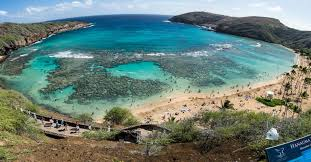
\includegraphics[width=8cm]{photos/hanauma.jpg}
\vfill
{\red{\Huge MAHALO!}}
\end{center}

\end{frame}

\begin{frame}
  \frametitle{This is my 100th trip to Knoxville}

\begin{center}


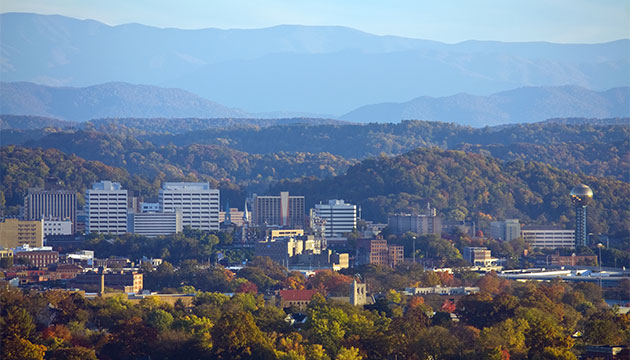
\includegraphics[width=4cm]{photos/knoxville.jpg} \hspace{0.5cm}
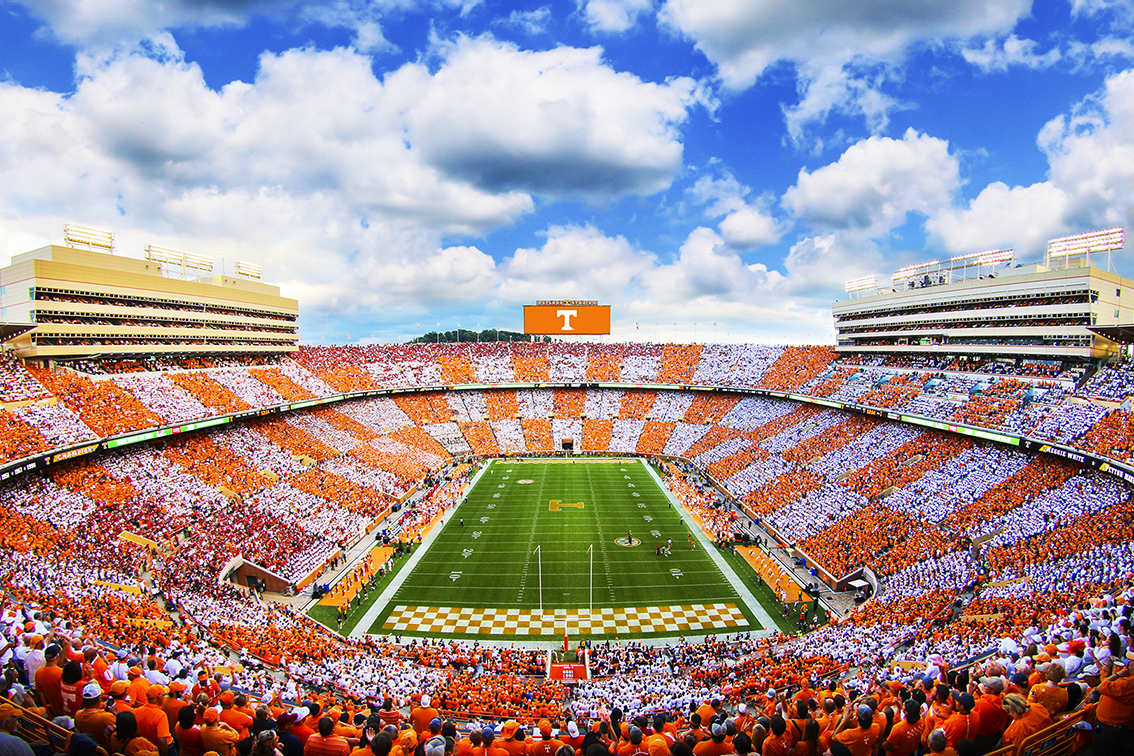
\includegraphics[width=3.7cm]{photos/neyland.jpg}\\

\vfill
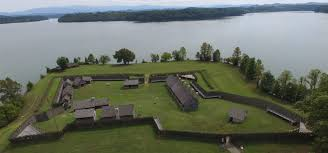
\includegraphics[width=4cm]{photos/fort-loudoun.jpg} \hspace{0.5cm}
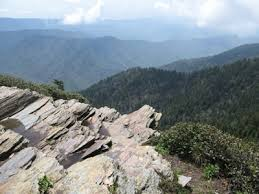
\includegraphics[width=3.5cm]{photos/mont-leconte.jpg}\

\vfill
{\red{\Huge THANK YE ALL!}}
\end{center}



\end{frame}


\begin{frame}
  \frametitle{This is my 1st seminar in Bordeaux}

\centering

%\onslide<1->{%
%\vspace*{-3cm}
\begin{myblock}{Olivier Beaumont}%

\vfill

%\onslide<2->

\vfill
{\red{\Huge MERCI GOPI!}}
\end{frame}

\end{document}
